\documentclass[a4paper]{article}
\usepackage[margin = 1 in]{geometry}
\usepackage{fancyhdr}
\usepackage{lastpage}
\usepackage{ctex}
\usepackage[utf8]{inputenc} % Required for inputting international characters
\usepackage[T1]{fontenc} % Output font encoding for international characters
\usepackage[sfdefault]{ClearSans} % Use the Clear Sans font (sans serif)
\usepackage{tocloft} 
\usepackage[hidelinks]{hyperref}
\usepackage{makecell}%导入表格宏包
\usepackage{bmpsize}
\usepackage{graphicx}
\usepackage{epstopdf}
\usepackage{caption}
\usepackage{enumitem}
\usepackage{float}
\usepackage{multirow}
\usepackage{makecell}

\pagestyle{fancy}
\lhead{\textsl{Team Project}}
\chead{}
\rhead{Page \thepage\ of \pageref{LastPage}}
\lfoot{}
\rfoot{}
\cfoot{}
\renewcommand{\headrulewidth}{0.4pt}
\renewcommand{\footrulewidth}{0pt}
\renewcommand{\cftsecleader}{\cftdotfill{\cftdotsep}}
\newcommand{\tabincell}[2]{\begin{tabular}{@{}#1@{}}#2\end{tabular}} %单元格内换行

\renewcommand*\contentsname{Table of Contents}

\begin{document}

%----------------------------------------------------------------------------------------
%	TITLE PAGE
%----------------------------------------------------------------------------------------

\begin{titlepage}
	
	\rule{\linewidth}{5pt}
	\raggedleft
	\fontsize{38pt}{50pt}\selectfont
    \textbf{\\Team Project\\}
    \fontsize{28pt}{60pt}\selectfont 
    for\\
    \fontsize{38pt}{60pt}\selectfont 
    \textbf{Milestone 1\\}
	
	\vfill % Space between the title box and author information
	
	%------------------------------------------------
	%	Author name and information
	%------------------------------------------------
	
	\parbox[t]{0.93\textwidth}{ % Box to inset this section slightly
		\raggedleft % Right align the text
		\large % Increase the font size
		{\Large By Team 23-22}\\[4pt] % Extra space after name
		Bogdan-Marian Gheorghe\_2329324\_bxg125\\
		Chance Egbon\_2194210\_cee010\\
		Gilead Bempah\_2296232\_gxb035\\
		Matthew Goulding\_2330080\_mxg183\\
		Samuel Okasia\_2345883\_sxo183\\
		Smit Navinkumar\_2327596\_sxn197\\
		Zijun Li\_2272583\_zxl183\\
	}
	
\end{titlepage}

\begin{center}
	\tableofcontents
	\addcontentsline{toc}{section}{Table of Contents}
\end{center}
\newpage

\section{S1 ranking}

{\noindent\begin{tabular}{|p{0.075\linewidth}|p{0.3\linewidth}|p{0.5\linewidth}|} 
	\hline
 \textbf{Rank} & \textbf{Name} & \textbf{Comments} \\
 \hline
 1 & Gilead Bempah						& The mockup fits well with the concept we are going for, as it blocks apps for a certain duration which helps with anti-procrastination. It clearly shows which apps are blocked and for how long. The persona is believable as it represents what a real student may be struggling with, for example spending too much time on social media and losing focus, and falling behind on work as a result. The persona is useful and relevant for the concept. The mockup is also very useful for the persona as it would block out the distracting apps (the persona has certain goals like improving focus)\\
 \hline
 2 & Samuel Okasia							& The Productivity Activity History records shows a graph, different screen section showing dates, times and subjects names, representing components of the to-do list and schedule features. This shows that the mock-up matched initial agreed format. The mock up bears similarities with the procrastinating features with its use of a clock system to keep track of how much time a user spends in a particular time it also clear that it links to the scheduler and the to do list. Although the mock up doesn’t offer no innovative feature as it is like existing solution, it looks good an it offers features that will be useful for the personas.\\
 \hline
 3 & Zijun Li									& The To-do list mock-up looks very straight forward and easy to use. It is self explanatory and user-friendly.  It allows you to set priority for your tasks which is very useful, also groups the daily tasks in different lists such as Entertainment, Study, Work. This grouping allows the user to better navigate through the tasks. I would suggest adding the option to add deadlines for different tasks and also adding a tick box to enable/disable email notifications for a specific task.\\
 \hline
\end{tabular}}

\newpage

{\small\noindent\begin{tabular}{|p{0.075\linewidth}|p{0.3\linewidth}|p{0.5\linewidth}|} 
\hline
 4 & Chance Egbon								& The diary mockup is well-suited to our goal of aiding productivity, as it allows users to organize and reflect on their daily activities. The use of color-coding for entries and categories facilitates quick reference and assists users in staying on track. The persona is realistic and relevant, depicting a typical individual struggling with time management and seeking an efficient way to manage their tasks. The persona adds value to the design by representing a broader audience. The mockup would be useful to the persona, allowing them to prioritize their daily tasks and track their progress towards their goals.\\
 \hline
 5 & Bogdan-Marian Gheorghe					& A very well thought out mock-up which links well to the projects concept by supplying an email overview of the user's schedule and tasks. The design of the feature is well executed with good aesthetics and dark mode has been considered for accessibility. It is slightly similar to other solutions so could be adapted maybe with links to the task/event that takes the user to that point on the app.\\
 \hline
 6 & Smit Navinkumar							& The scheduler mockup looks clean and easy to use. The color coding of the different tasks provides a quick visual reference for the user. It would be helpful to include a feature that allows the user to filter tasks by category or due date.It would be beneficial to add more details to the persona to make it more real and representative of a diverse range of users. Consider including additional information such as the individual's age, profession, interests, and technology proficiency. This would help ensure that the design meets the need and expectations of a broader audience.\\
 \hline
 7 & Matthew Goulding							& The mock-up is quite simple to comprehend and also mode sensitive. While using Chrome in dark mode, the typeface is white with a black backdrop, making it more aesthetically pleasing than when using Chrome in light mode, which has black text on a grey background. The design of the timer is a little rudimentary, therefore it has room for improvement; consequently, improving the GUI would be appreciated. Moreover, you could combine setting a timeframe with developing a character by having checkboxes that allow users to select which task they wish to do.\\
 \hline
\end{tabular}}

\newpage

\section{Agreed, coherent project concept \& personas \& mockups}

\subsection{Project concept}

Our project is a web-based application that helps with time management. It combines features of a scheduler and a to-do list, and also provides email notifications. With the anti-procrastination feature, you can control your own access to websites once you activate it. In addition, the application includes a timer and alarm to help you stay on track. The Diary feature allows you to add more details about upcoming events. The application also includes productivity analysis tools to help you track your progress and review your history.
\par
A scheduler is a feature of a time management application that allows you to view and manage your schedule. It provides a calendar view that displays your daily, weekly, or monthly events, allowing you to see your availability and plan your activities accordingly. You can also add, edit, and delete events in the scheduler, and set reminders or notifications to help you stay on track with your schedule.
\par
The to-do list feature allows users to create and organize tasks they need to complete. Users can set add sub-tasks, categorize tasks, and prioritize them. The to-do list can help users focus on important tasks and keep track of what needs to be done, providing a clear overview of their day or week.
\par
The anti-procrastination feature helps users avoid distractions by restricting their access to certain websites or apps during designated work times. User can set the blocking time to the particular webside(Blacklist) or set the avaliable website (Whitelist)
\par
The diary is designed to help users keep track of their thoughts and ideas about their day.  A diary can be used to record daily activities, emotions, and reflections, which can be used to better understand one's behavior and habits.
\par
The alarm/timer feature allows users to set reminders for important events or tasks. Users can set a specific time for the alarm or timer to go off.
\par
The email notification allows the user to receive notifications and reminders about important events or tasks via email. The user can add their email to the setting part and the system will send the mail when there are events automatically.
\par
The History feature provides a way to track and analyze one's productivity over time. User can check the total saved time and the time using the Time Management application.

\subsection{mockups}

\subsubsection{Scheduler}

\begin{figure}[H] %H为当前位置,!htb为忽略美学标准,htbp为浮动图形
	\centering %图片居中
	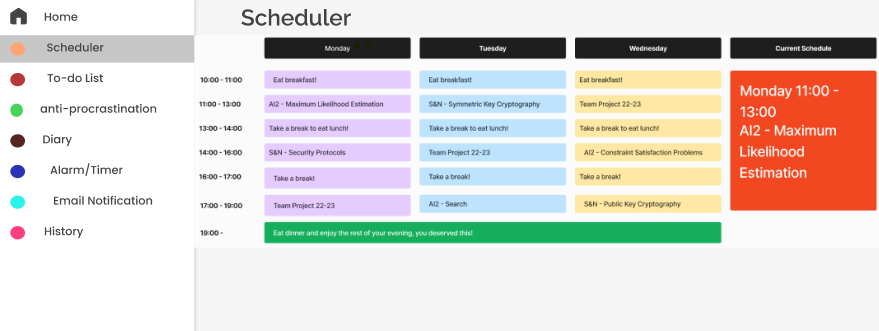
\includegraphics[width=1\textwidth]{./images/Mockup_Scheduler.png} %插入图片,[]中设置图片大小,{}中是图片文件名
	\caption*{Mockup: Scheduler} %最终文档中希望显示的图片标题
	\label{Fig.Scheduler} %用于文内引用的标签
\end{figure}

\subsubsection{To-do List}

\begin{figure}[H] %H为当前位置,!htb为忽略美学标准,htbp为浮动图形
	\centering %图片居中
	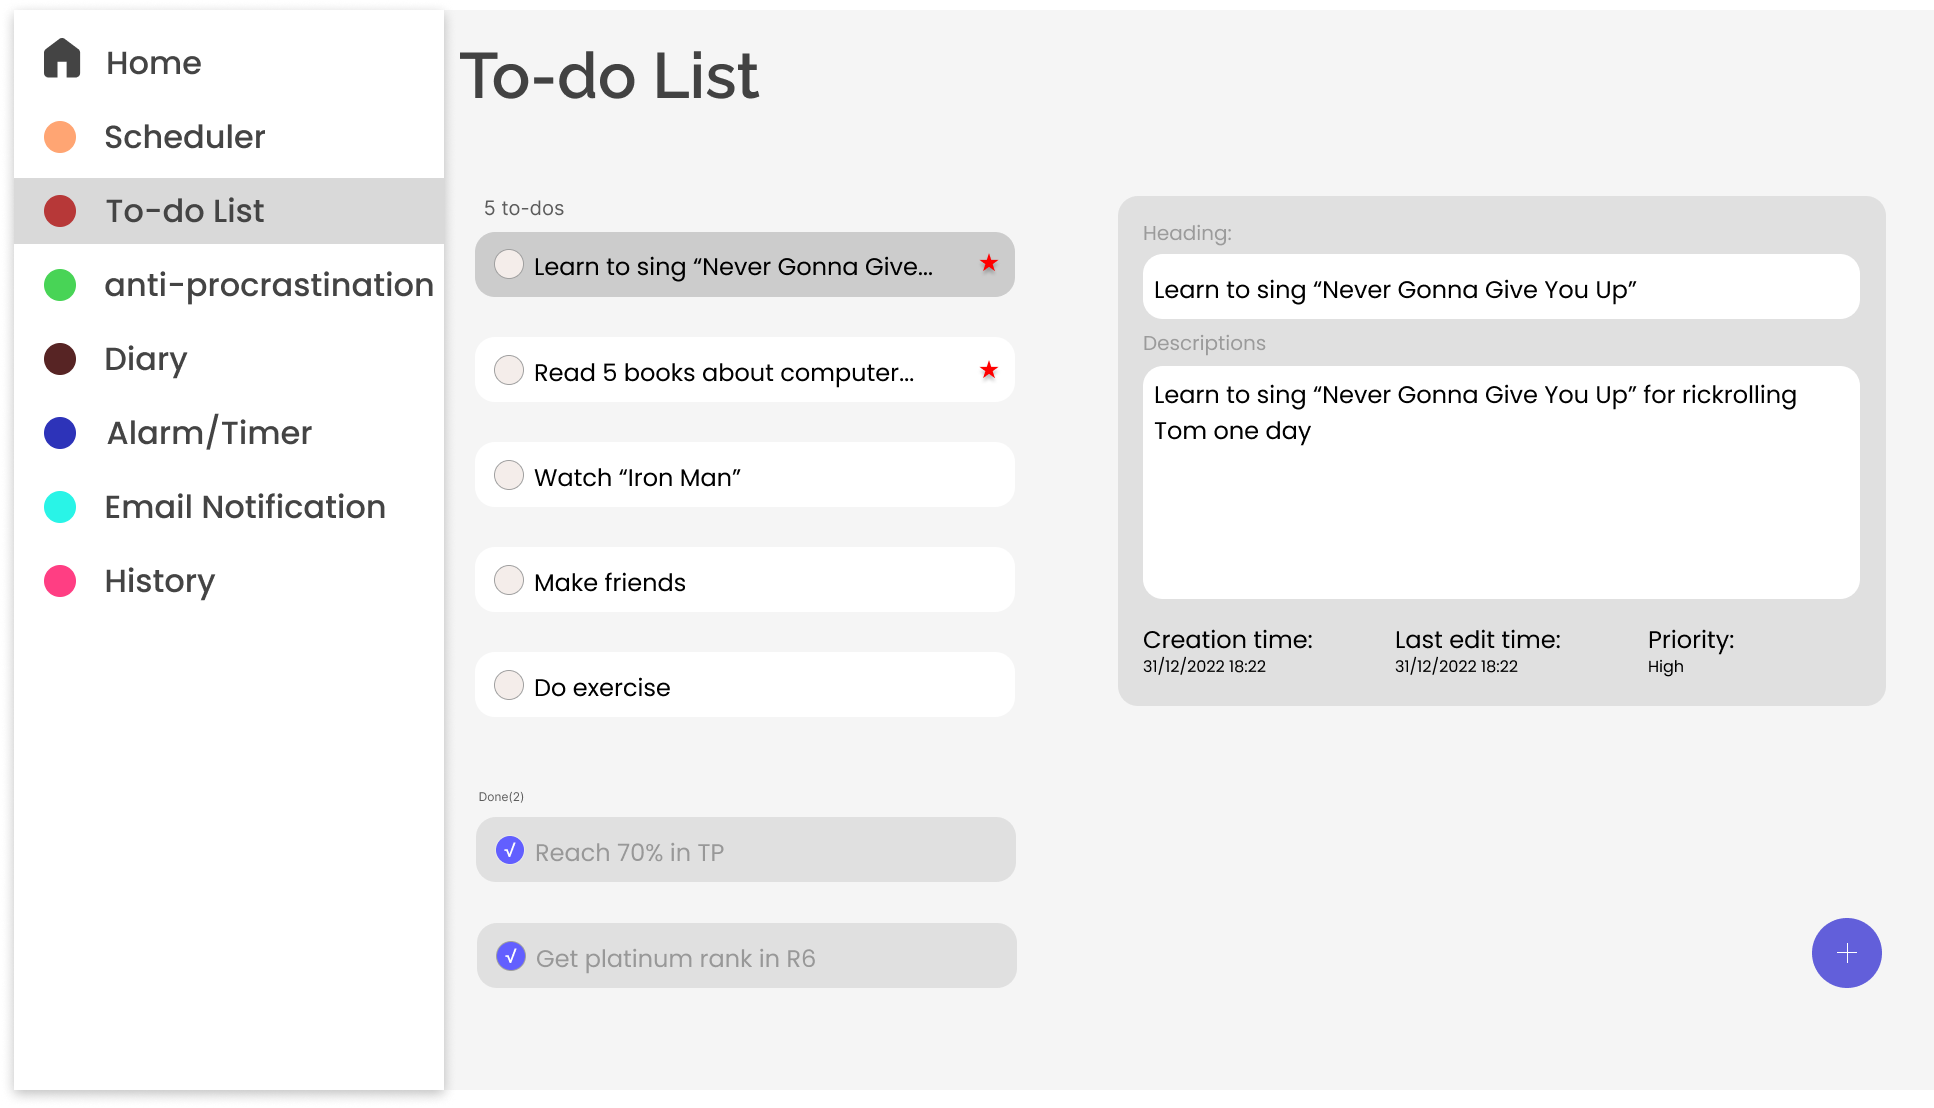
\includegraphics[width=1\textwidth]{./images/Mockup_Todo_list.png} %插入图片,[]中设置图片大小,{}中是图片文件名
	\caption*{Mockup: To-do List} %最终文档中希望显示的图片标题
	\label{Fig.todolist} %用于文内引用的标签
\end{figure}


\subsubsection{Anti-procrastination}

\begin{figure}[H] %H为当前位置,!htb为忽略美学标准,htbp为浮动图形
	\centering %图片居中
	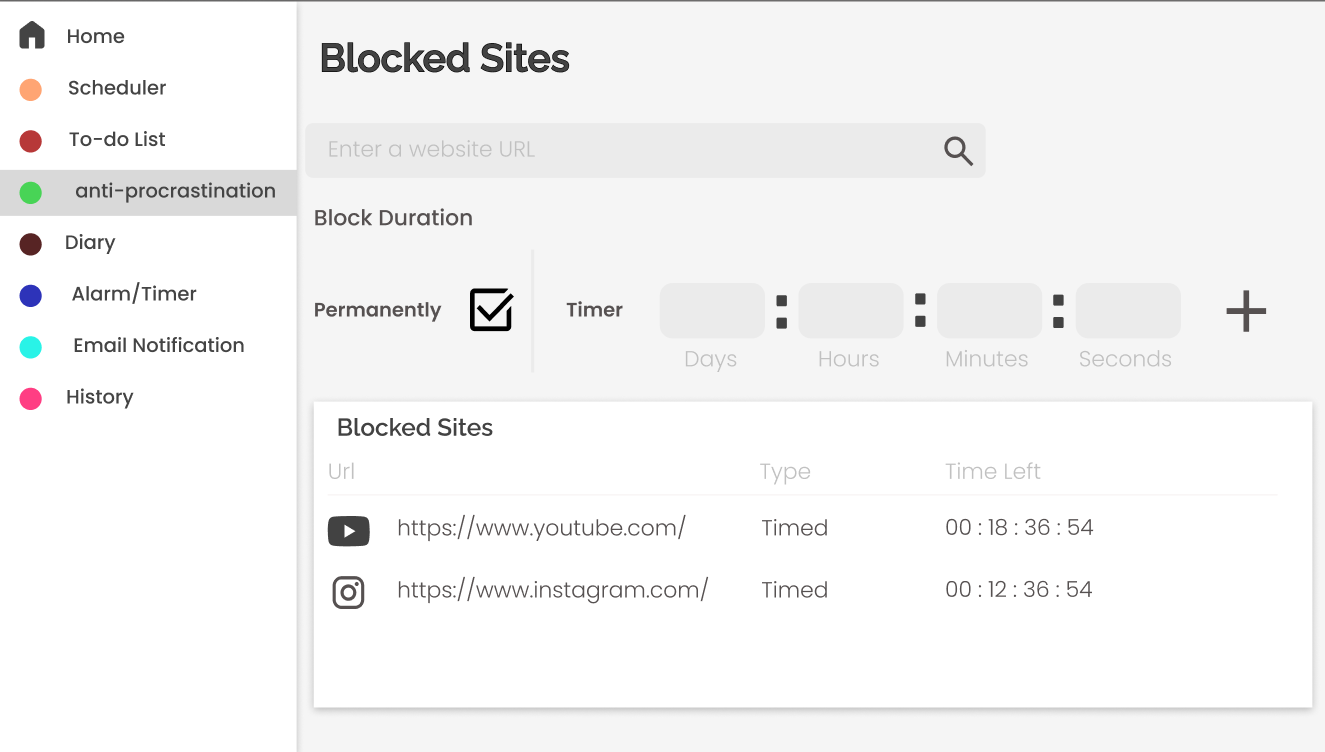
\includegraphics[width=1\textwidth]{./images/Mockup_Anti-procrastination.png} %插入图片,[]中设置图片大小,{}中是图片文件名
	\caption*{Mockup: Anti-procrastination} %最终文档中希望显示的图片标题
	\label{Fig.Anti-procrastination} %用于文内引用的标签
\end{figure}

\subsubsection{Diary}

\begin{figure}[H] %H为当前位置,!htb为忽略美学标准,htbp为浮动图形
	\centering %图片居中
	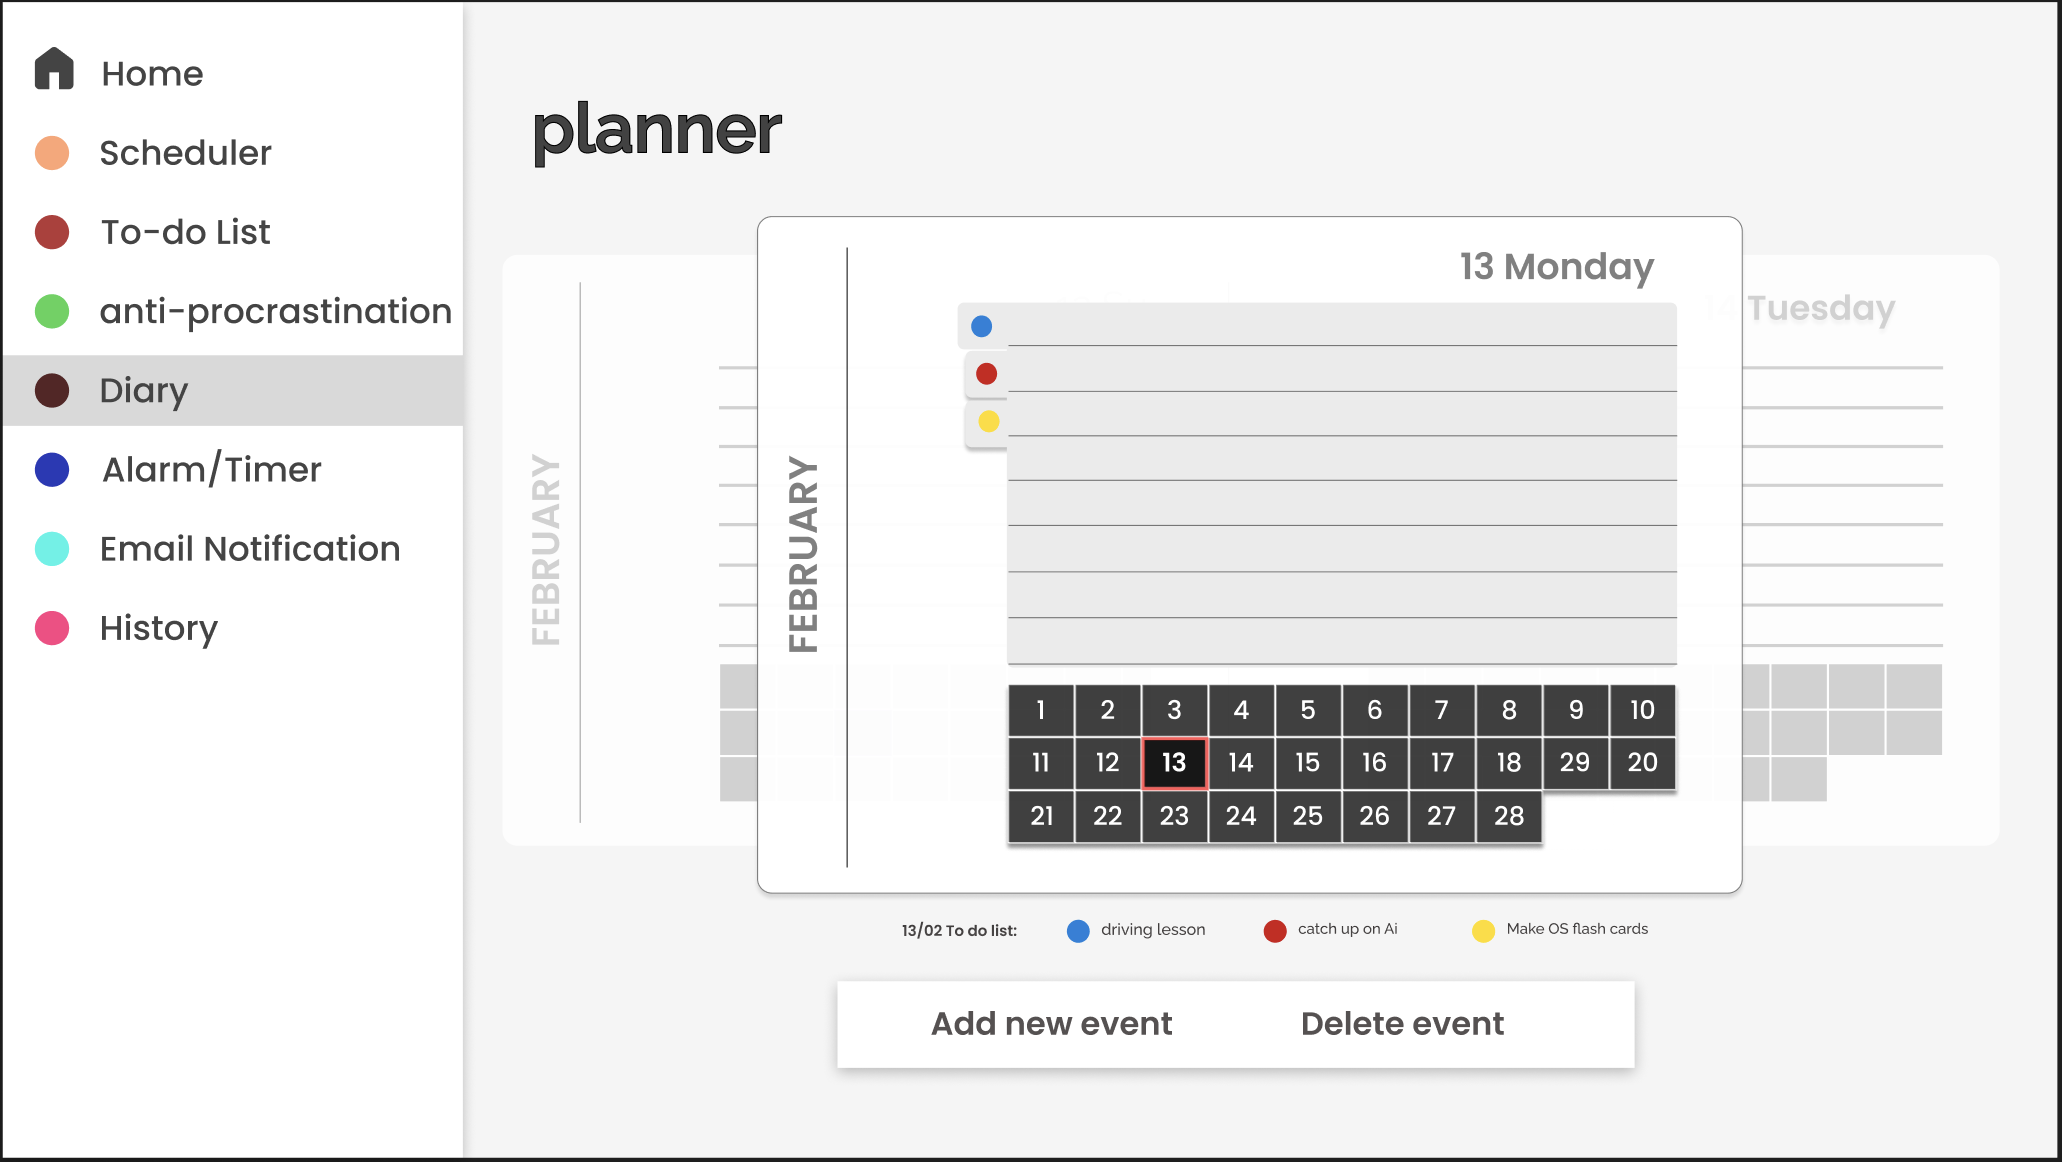
\includegraphics[width=1\textwidth]{./images/Mockup_Diary.jpg} %插入图片,[]中设置图片大小,{}中是图片文件名
	\caption*{Mockup: Diary} %最终文档中希望显示的图片标题
	\label{Fig.Diary} %用于文内引用的标签
\end{figure}

\subsubsection{Alarm/Timer}

\begin{figure}[H] %H为当前位置,!htb为忽略美学标准,htbp为浮动图形
	\centering %图片居中
	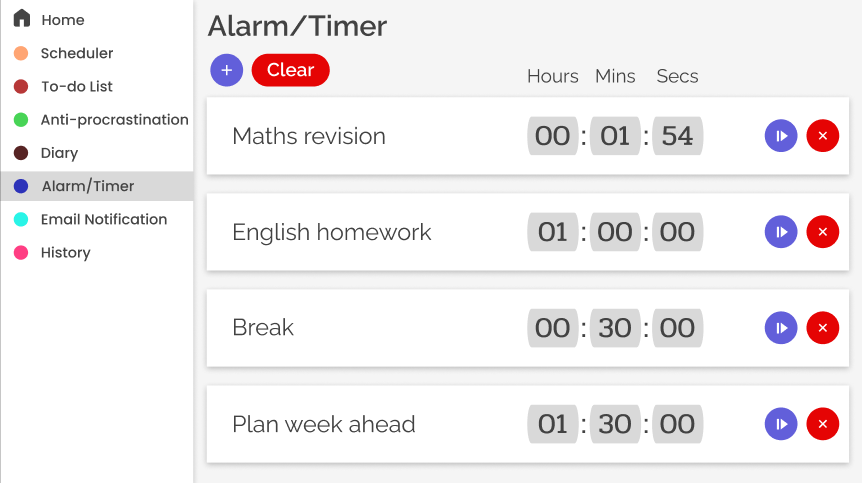
\includegraphics[width=1\textwidth]{./images/Mockup_AlarmTimer.png} %插入图片,[]中设置图片大小,{}中是图片文件名
	\caption*{Mockup: Alarm} %最终文档中希望显示的图片标题
	\label{Fig.Alarm} %用于文内引用的标签
\end{figure}

\subsubsection{History}

\begin{figure}[H] %H为当前位置,!htb为忽略美学标准,htbp为浮动图形
	\centering %图片居中
	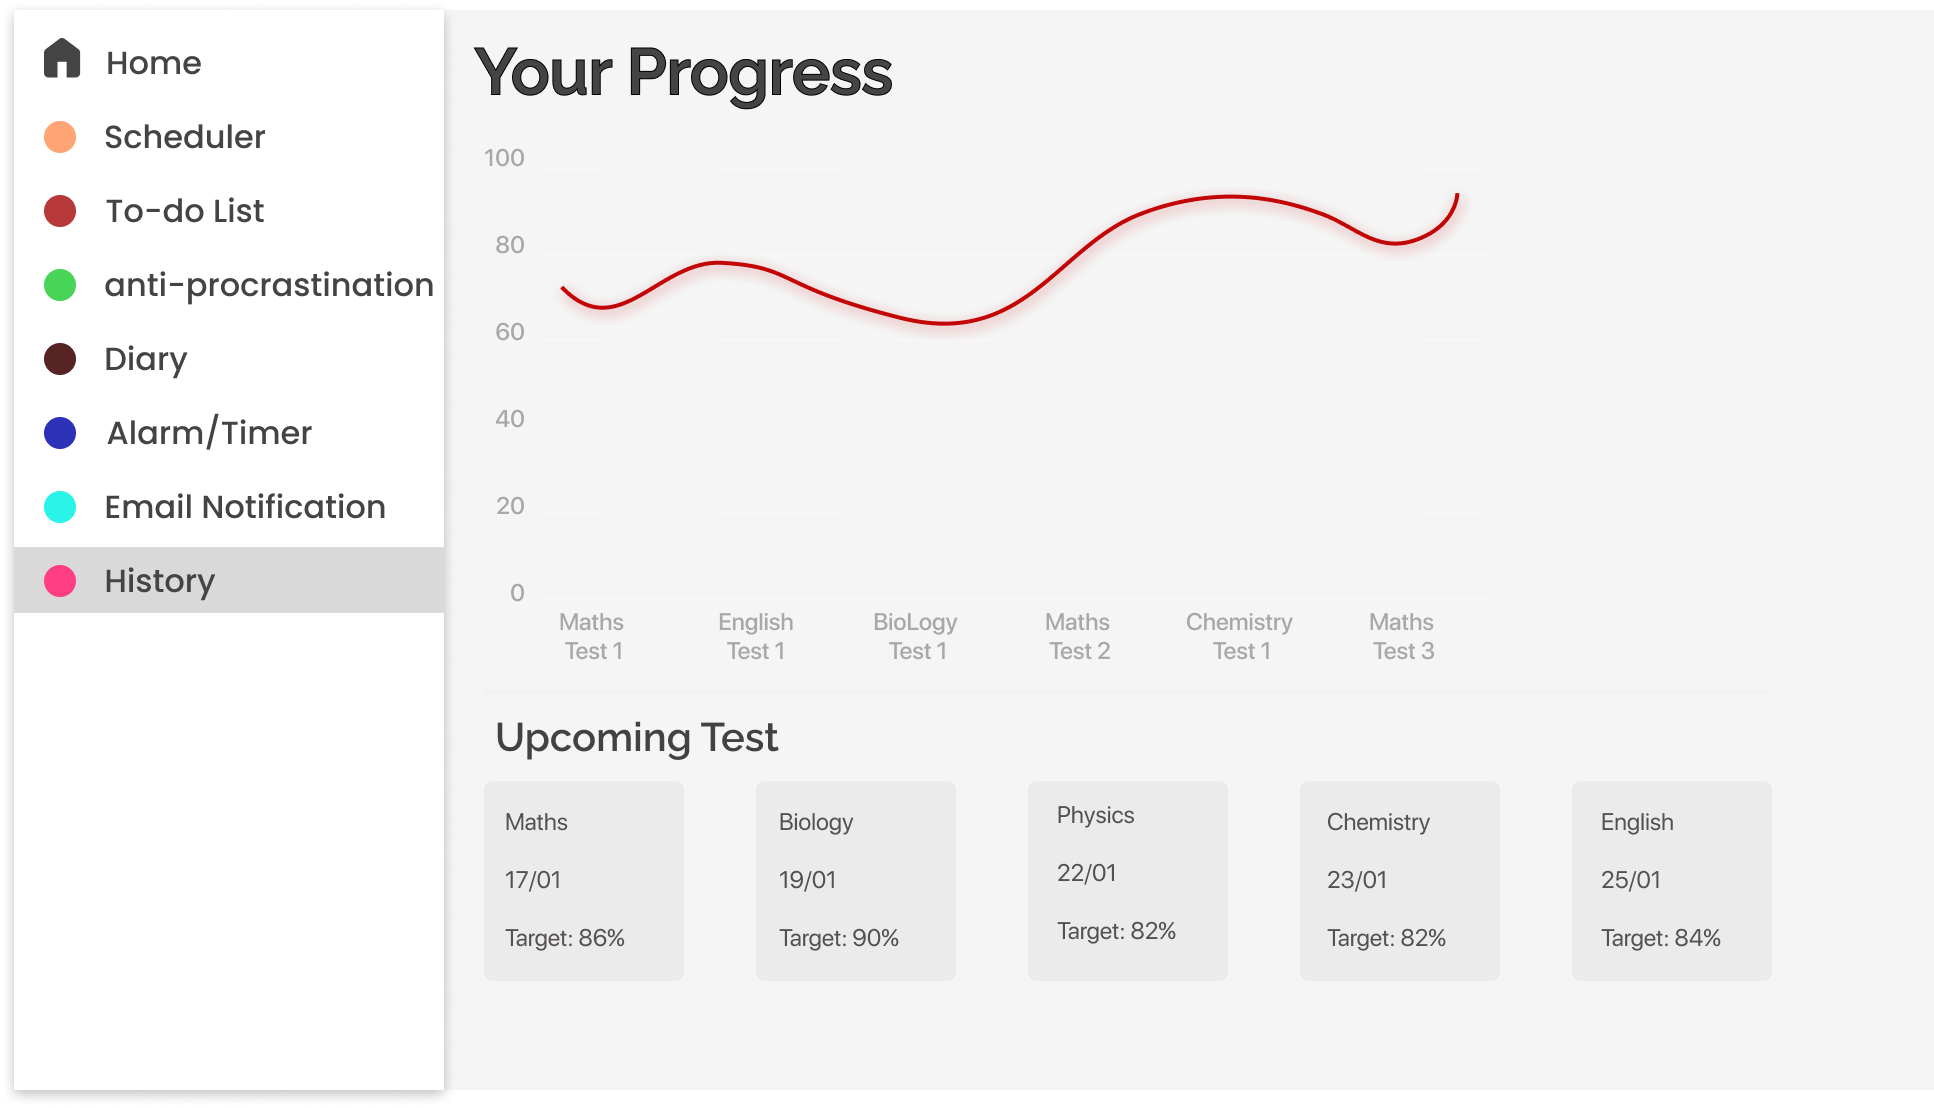
\includegraphics[width=1\textwidth]{./images/Mockup_History.png} %插入图片,[]中设置图片大小,{}中是图片文件名
	\caption*{Mockup: History} %最终文档中希望显示的图片标题
	\label{Fig.History} %用于文内引用的标签
\end{figure}

\subsubsection{Email notifications}

\begin{figure}[H] %H为当前位置,!htb为忽略美学标准,htbp为浮动图形
	\centering %图片居中
	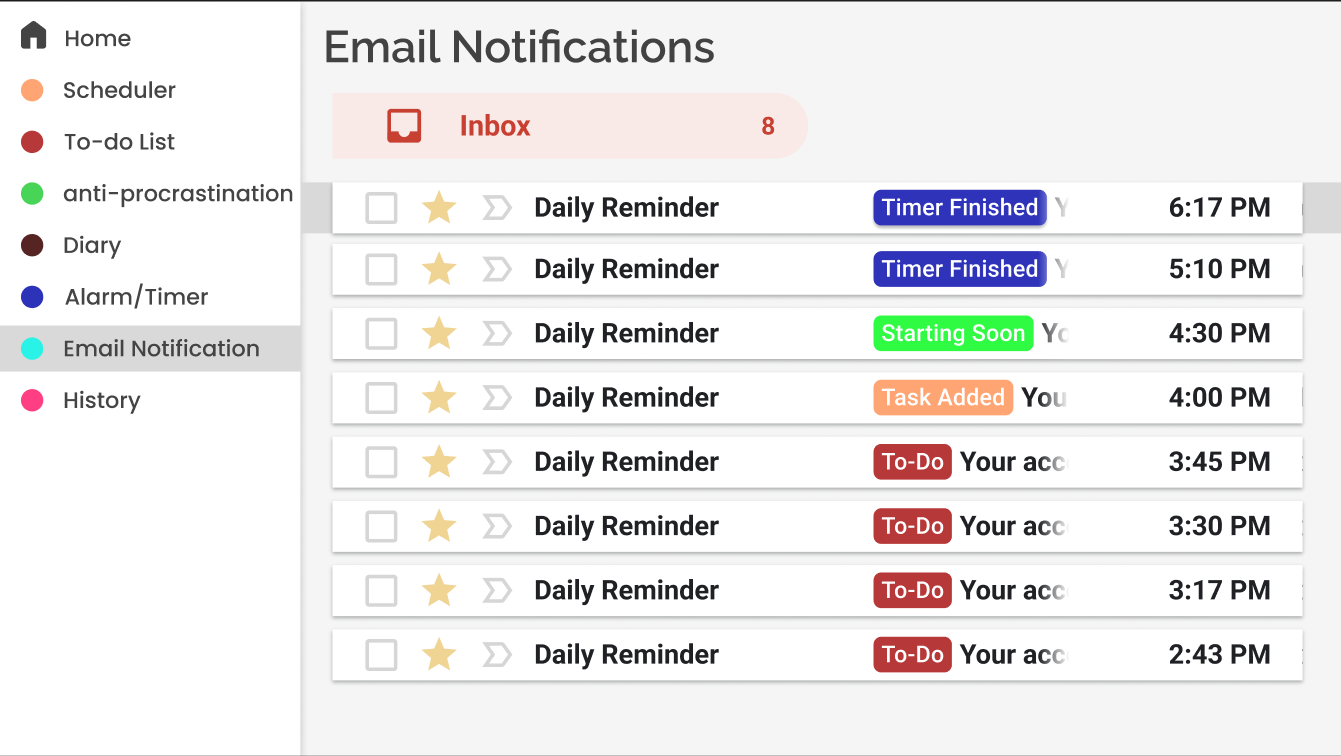
\includegraphics[width=1\textwidth]{./images/Mockup_Email_normal.png}
	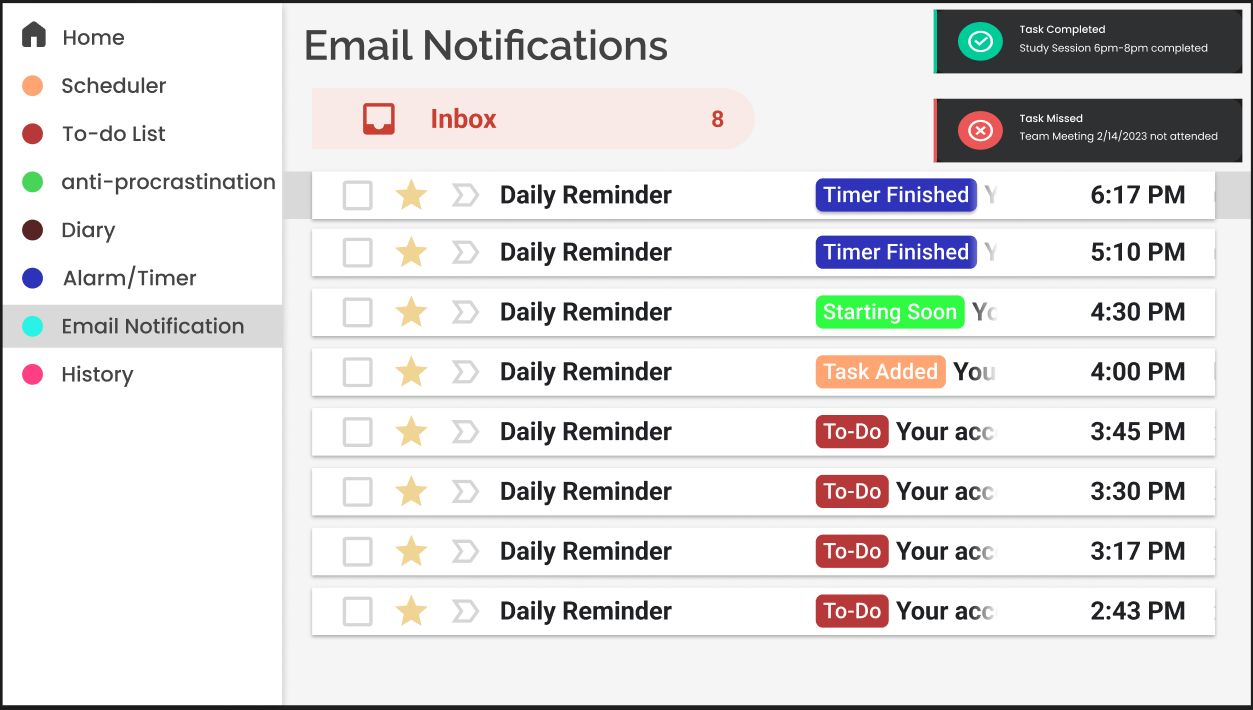
\includegraphics[width=1\textwidth]{./images/Mockup_Email.png} %插入图片,[]中设置图片大小,{}中是图片文件名
	\caption*{Mockup: Email notification} %最终文档中希望显示的图片标题
	\label{Fig.Email} %用于文内引用的标签
\end{figure}

\subsection{Persona}

\begin{figure}[H] %H为当前位置,!htb为忽略美学标准,htbp为浮动图形
	\centering %图片居中
	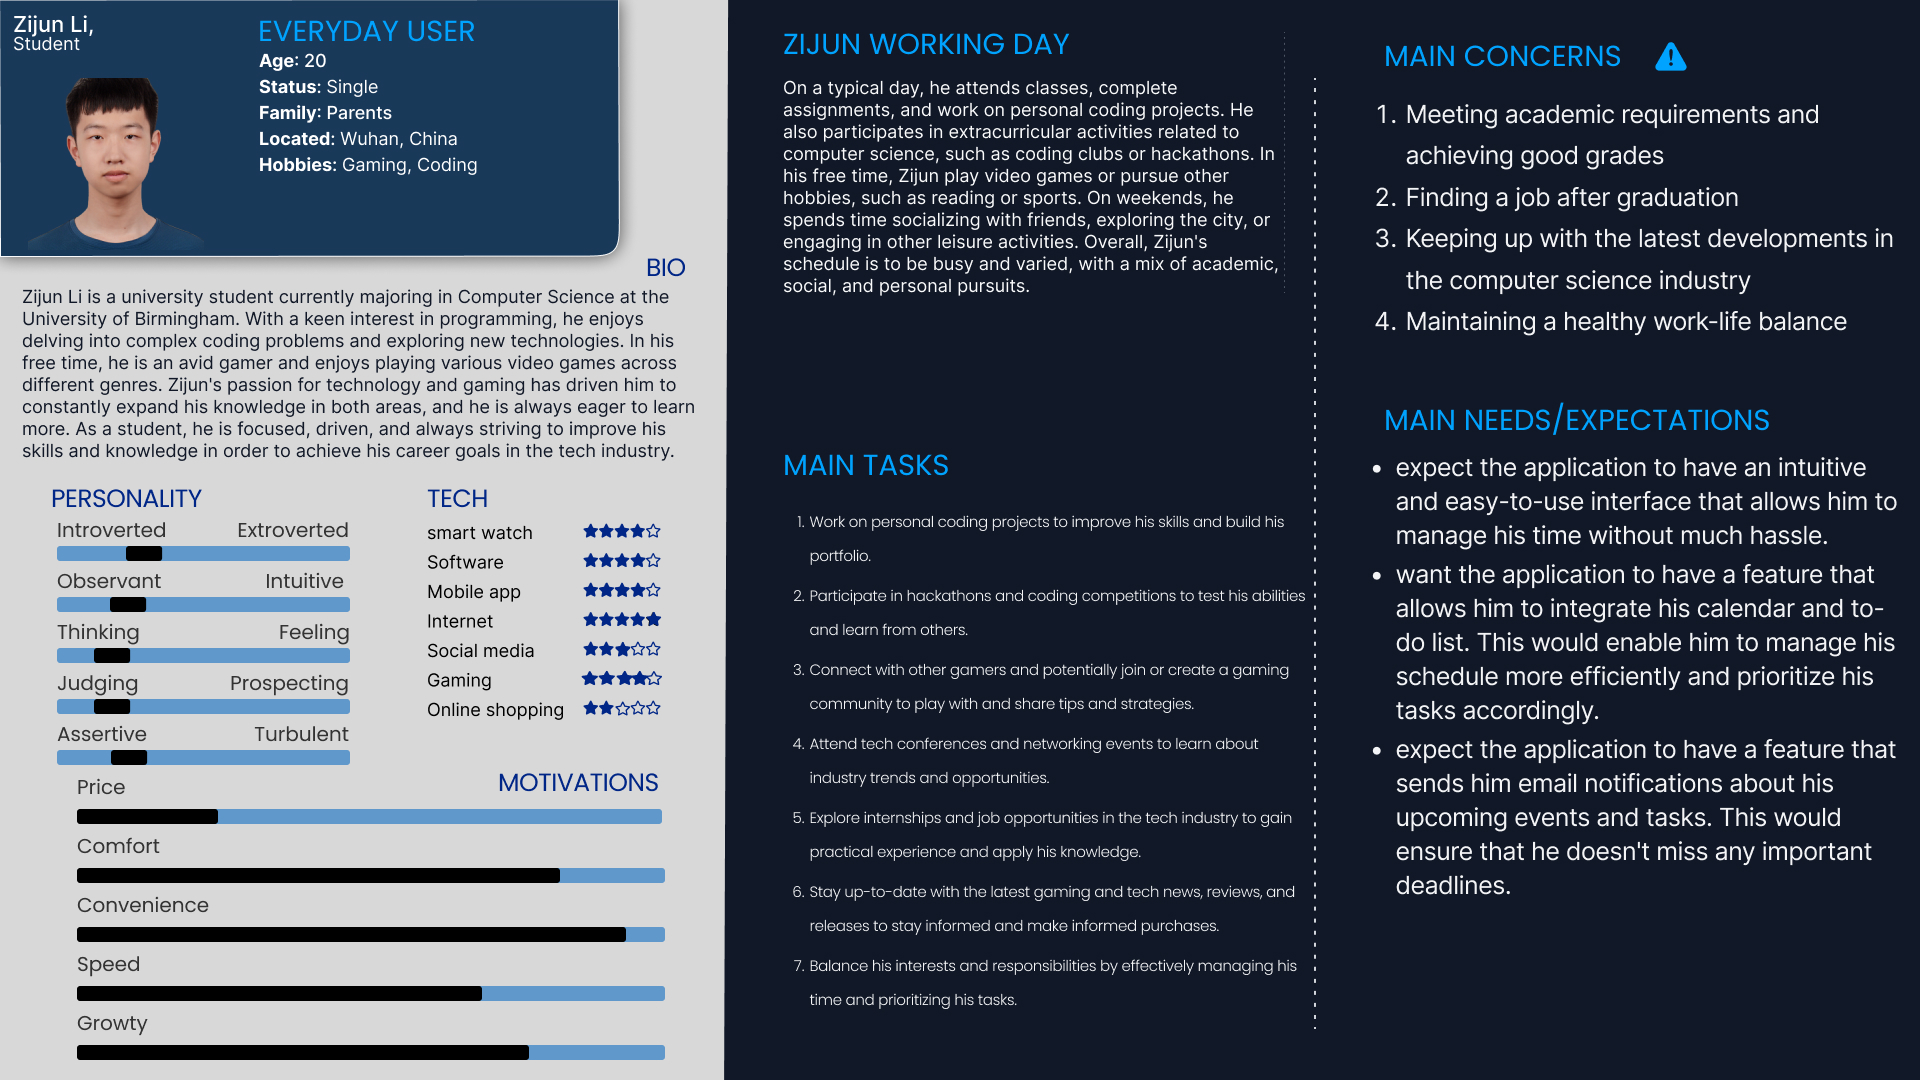
\includegraphics[width=1\textwidth]{./images/Persona_Zijun.jpg} %插入图片,[]中设置图片大小,{}中是图片文件名
	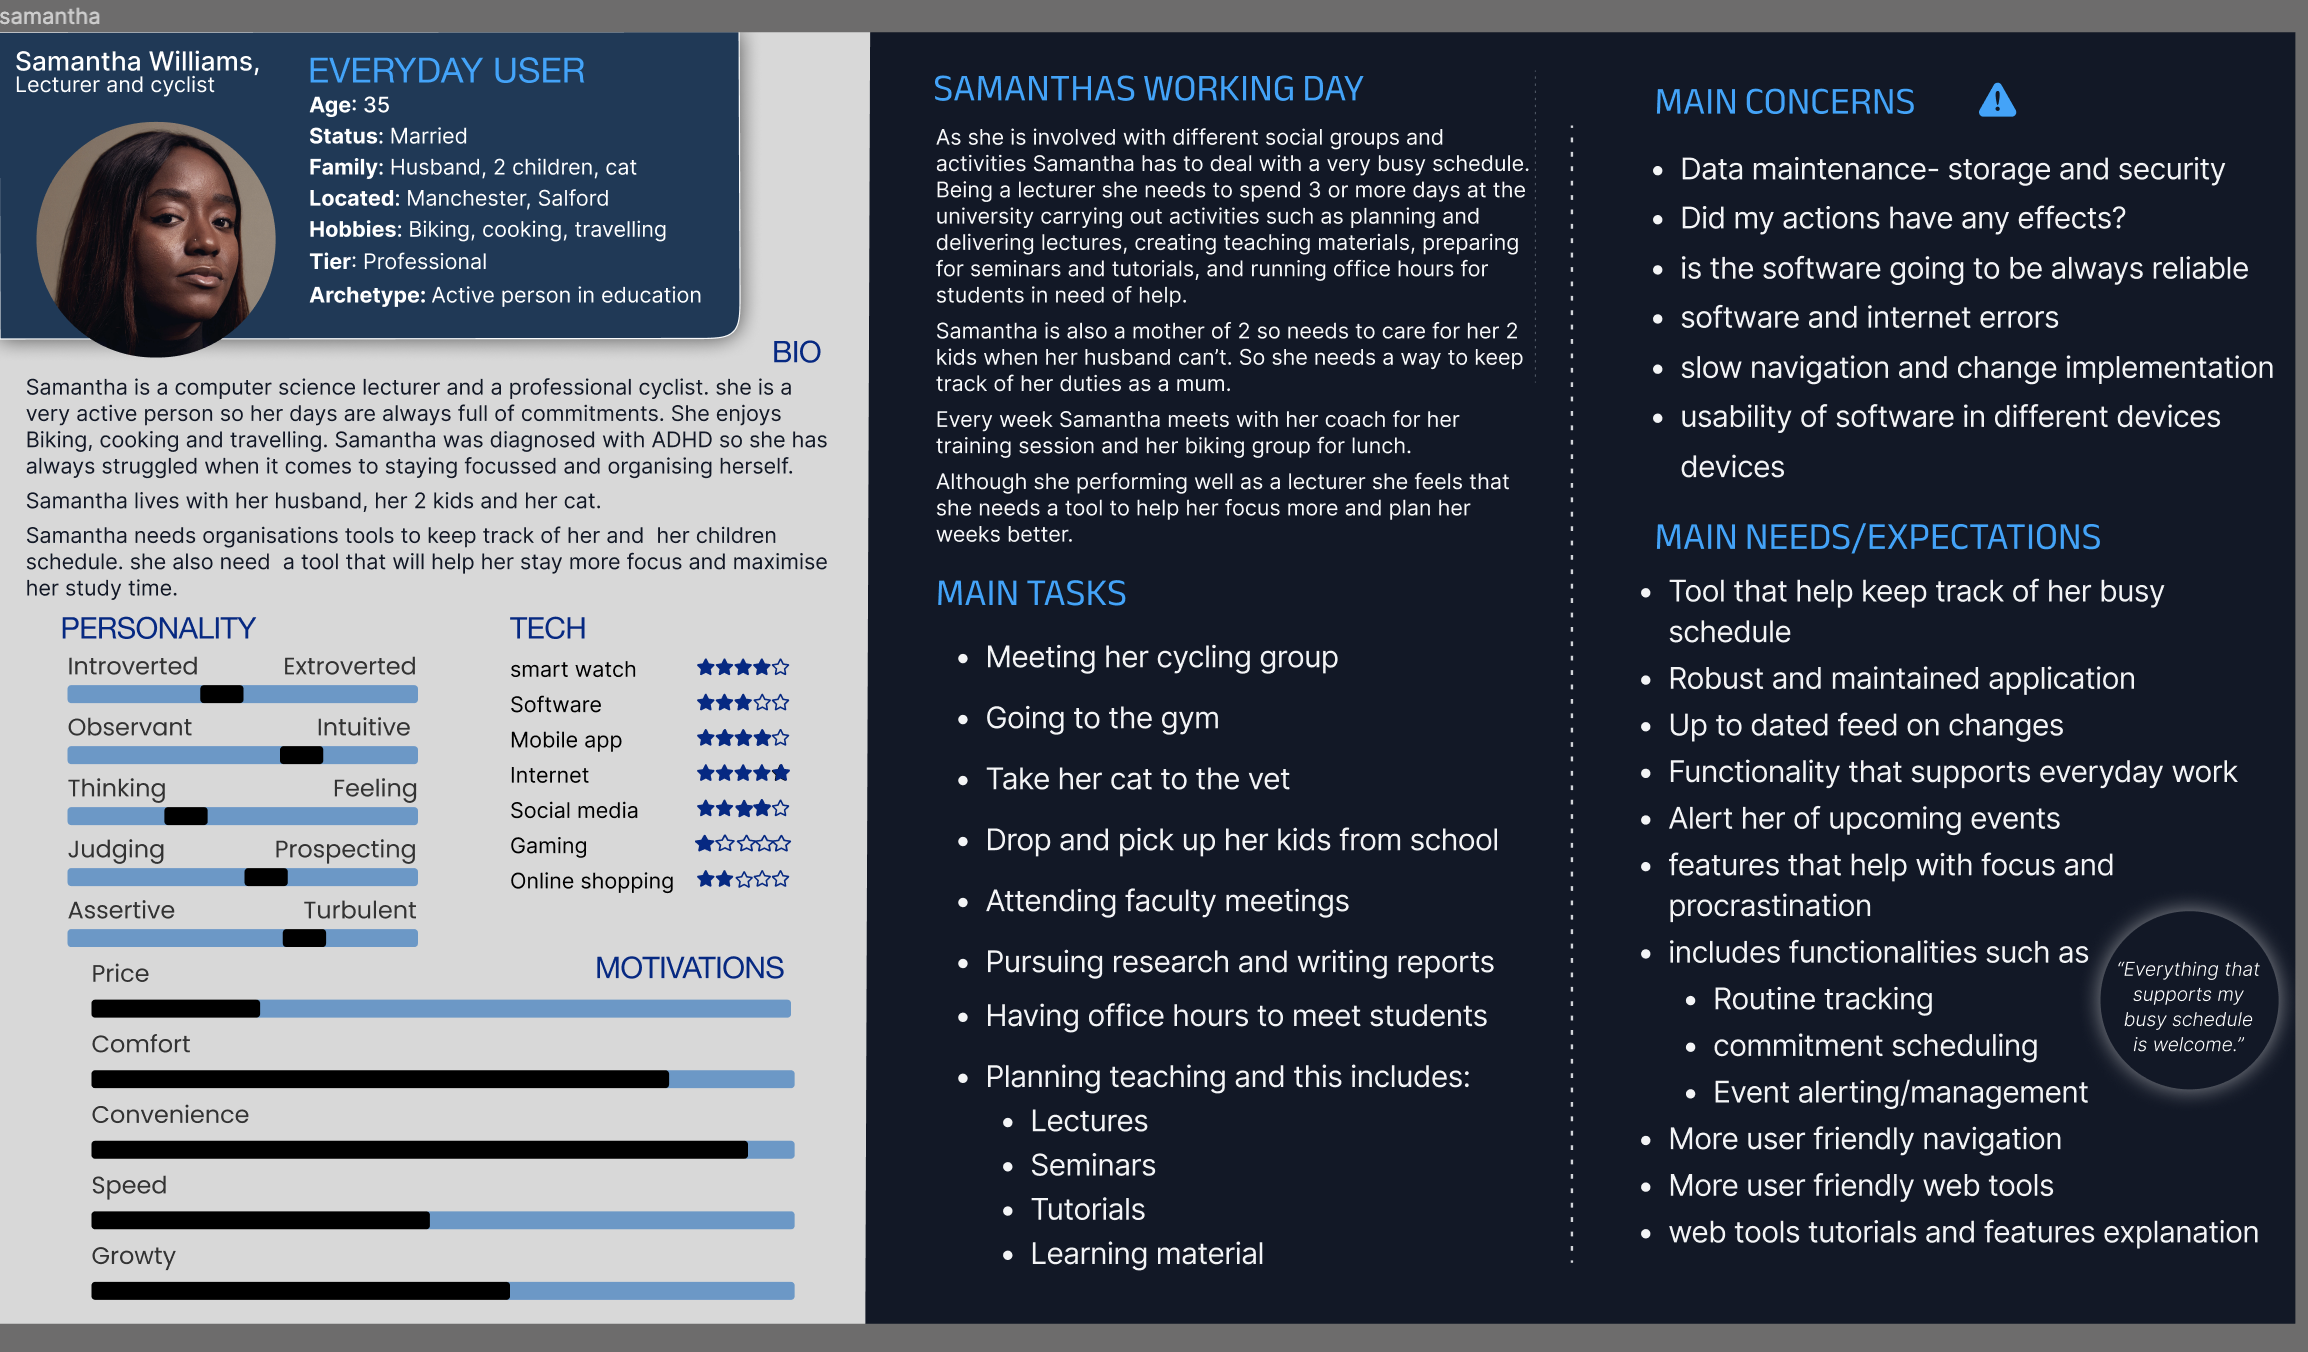
\includegraphics[width=1\textwidth]{./images/Persona_Chance.jpg}
	\caption*{} %最终文档中希望显示的图片标题
	\label{Fig.Personas1} %用于文内引用的标签
\end{figure}

\newpage

\begin{figure}[H] %H为当前位置,!htb为忽略美学标准,htbp为浮动图形
	\centering %图片居中
	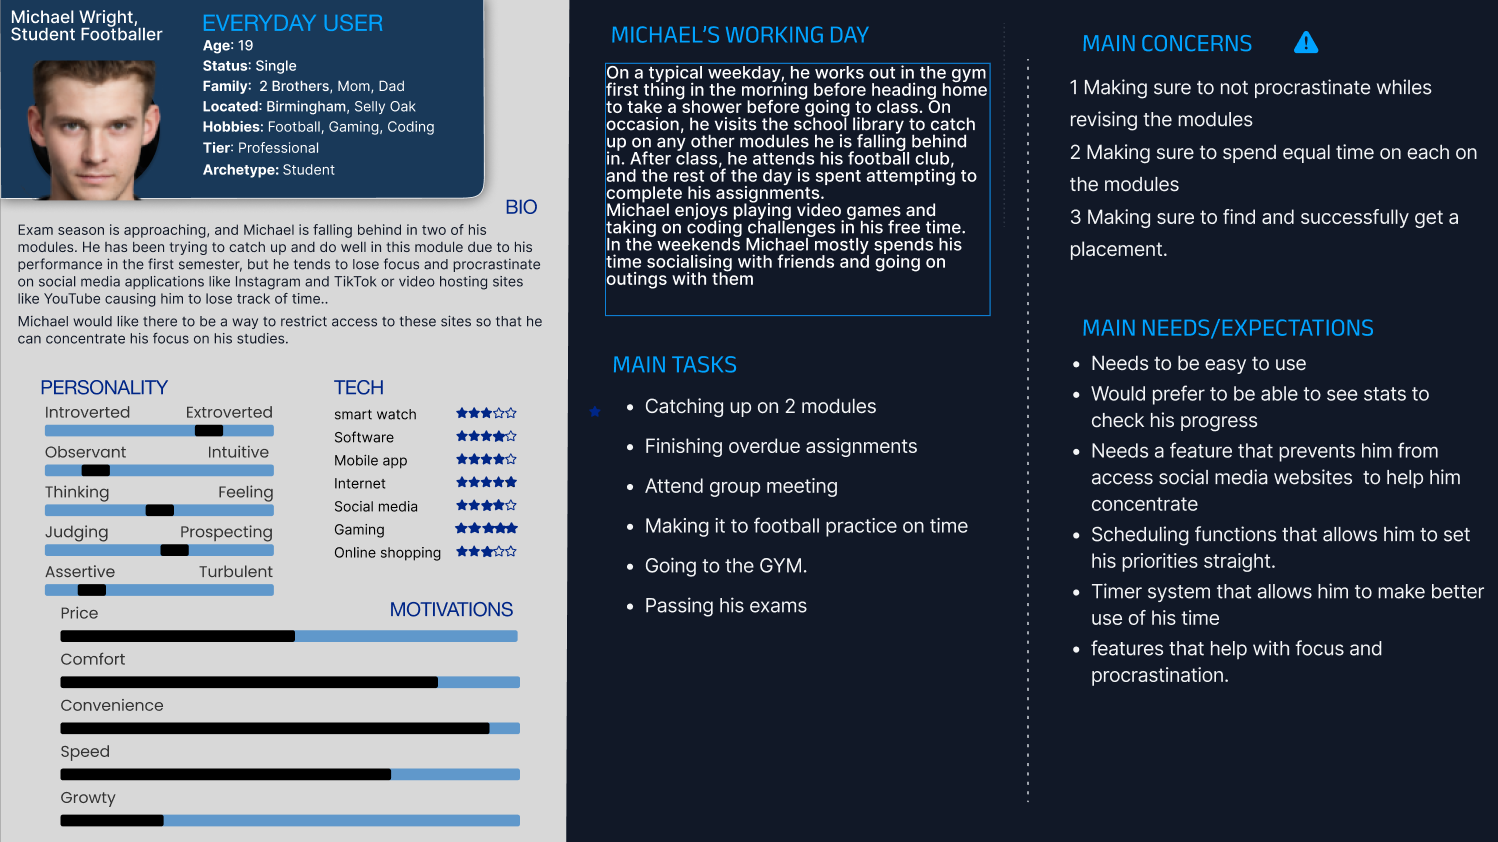
\includegraphics[width=1\textwidth]{./images/Persona_Gilead.png} %插入图片,[]中设置图片大小,{}中是图片文件名
	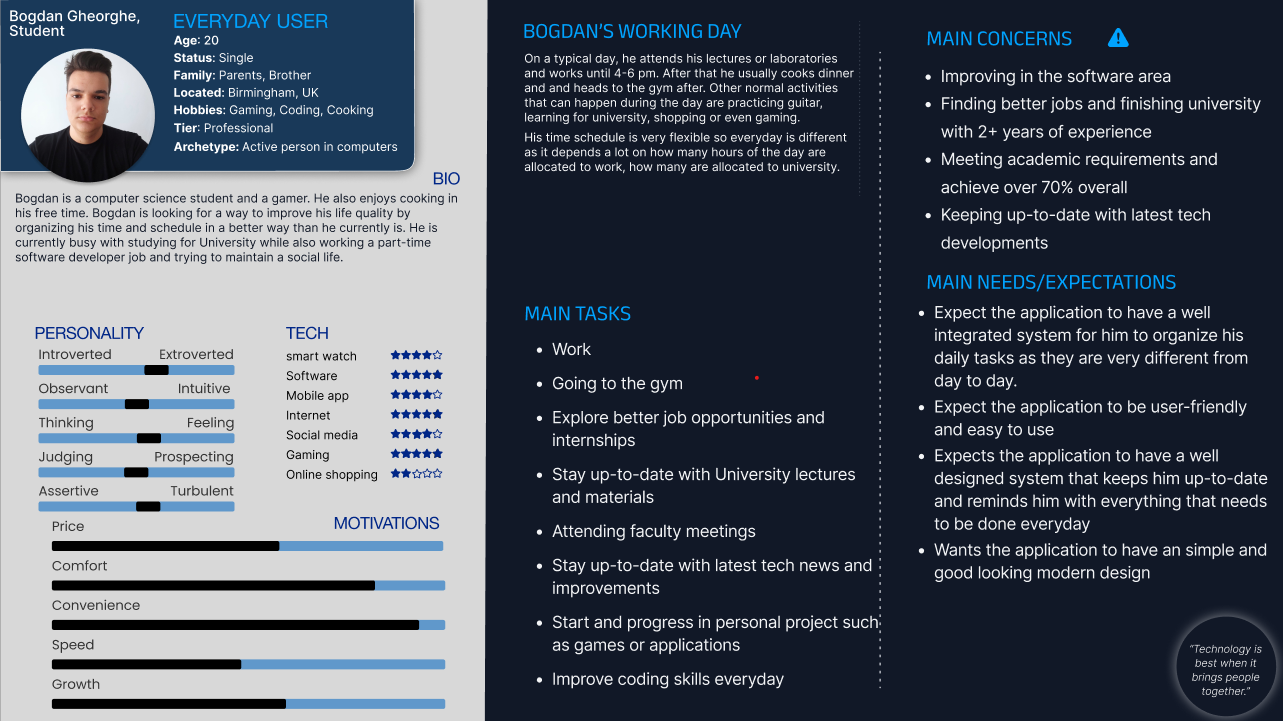
\includegraphics[width=1\textwidth]{./images/Persona_Bogdan.png}
	\caption*{} %最终文档中希望显示的图片标题
	\label{Fig.Persona2} %用于文内引用的标签
\end{figure}

\begin{figure}[H] %H为当前位置,!htb为忽略美学标准,htbp为浮动图形
	\centering %图片居中
	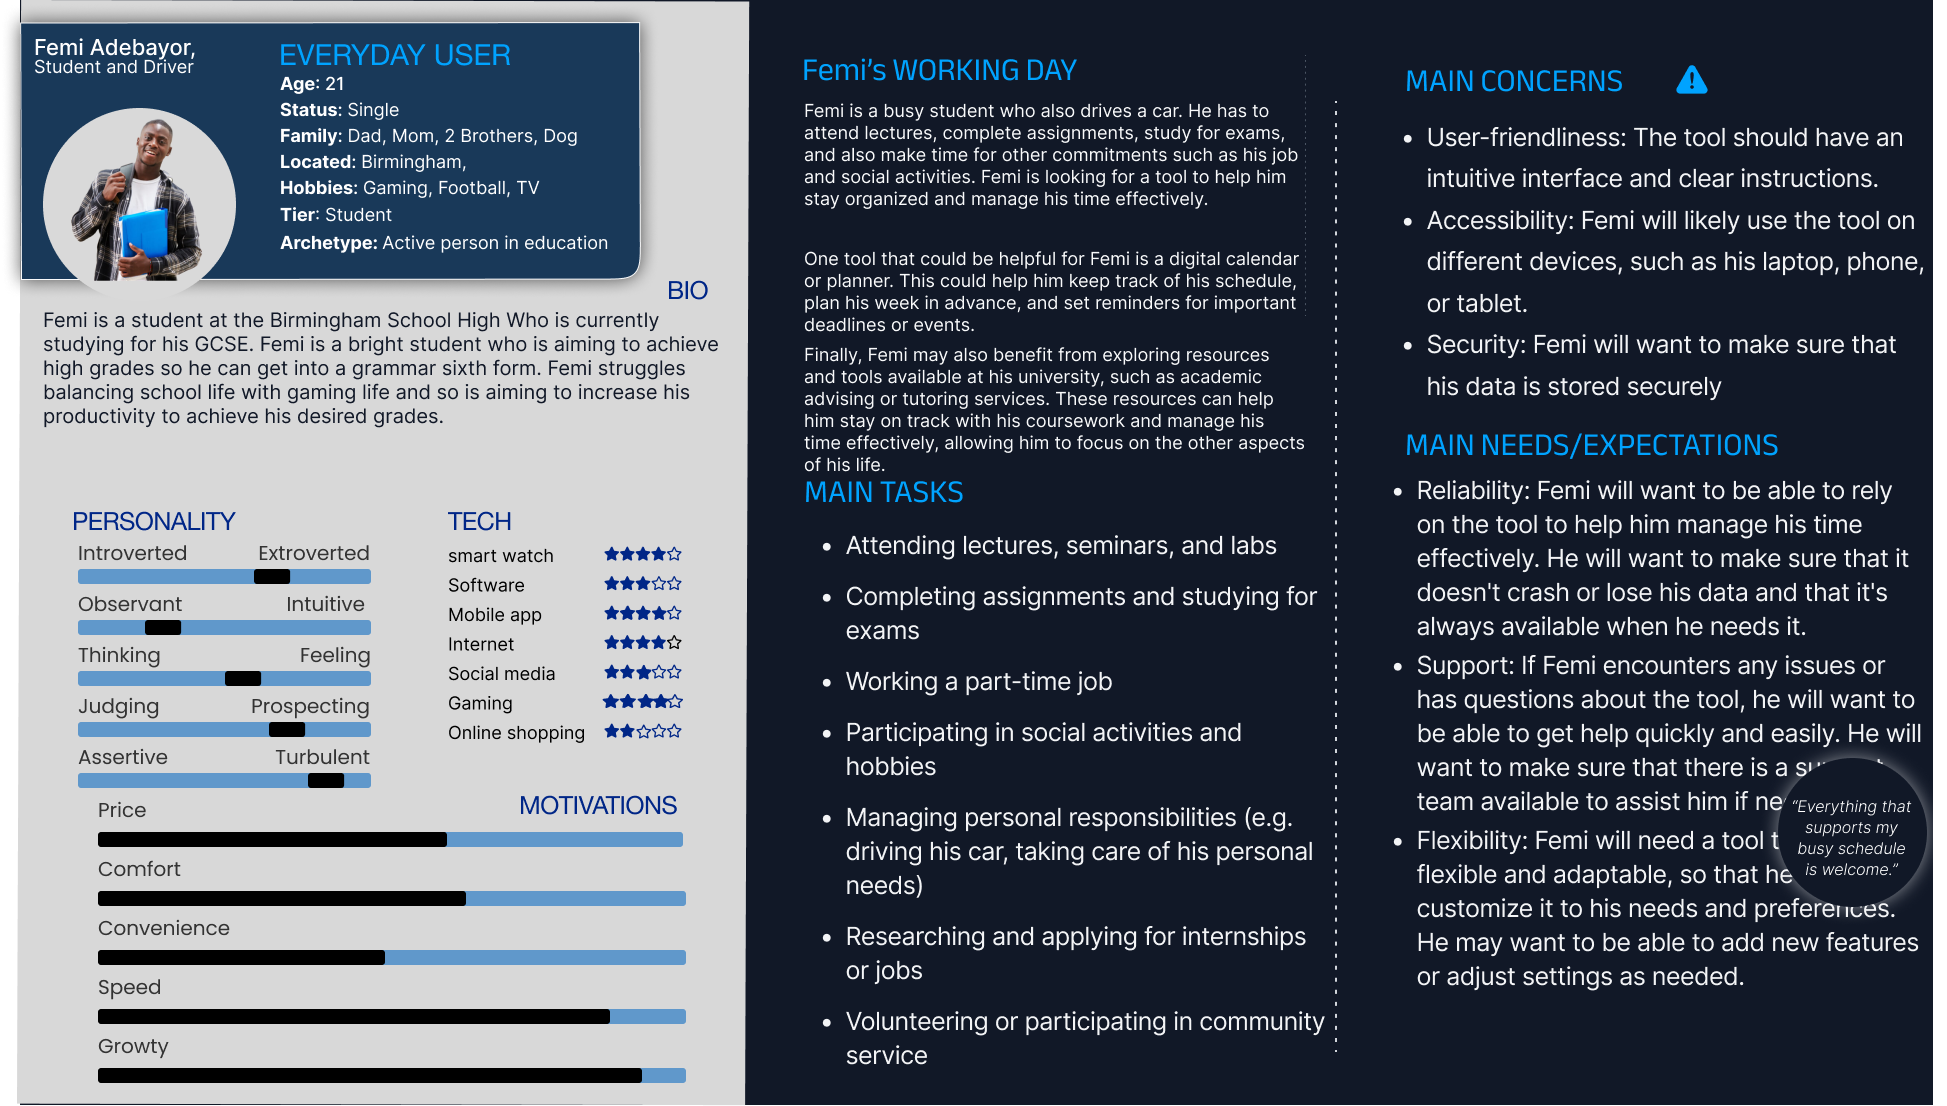
\includegraphics[width=0.92\textwidth]{./images/Persona_Samuel.jpg}
	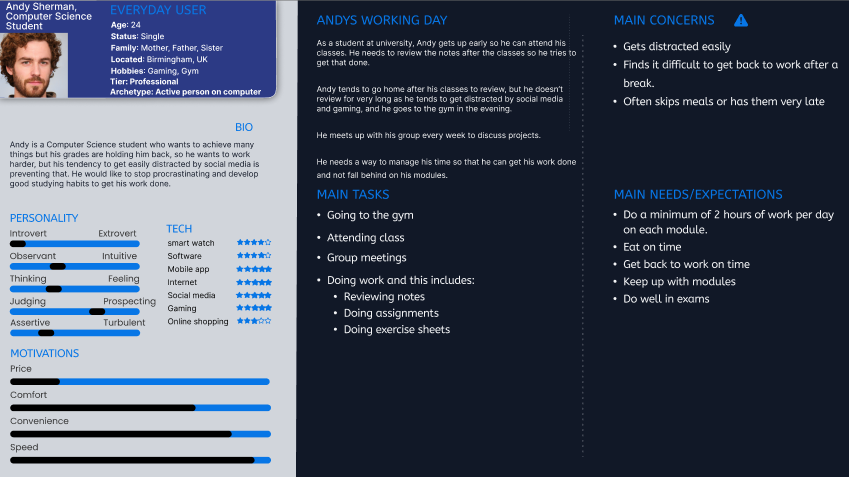
\includegraphics[width=0.92\textwidth]{./images/Persona_Smit.png}
	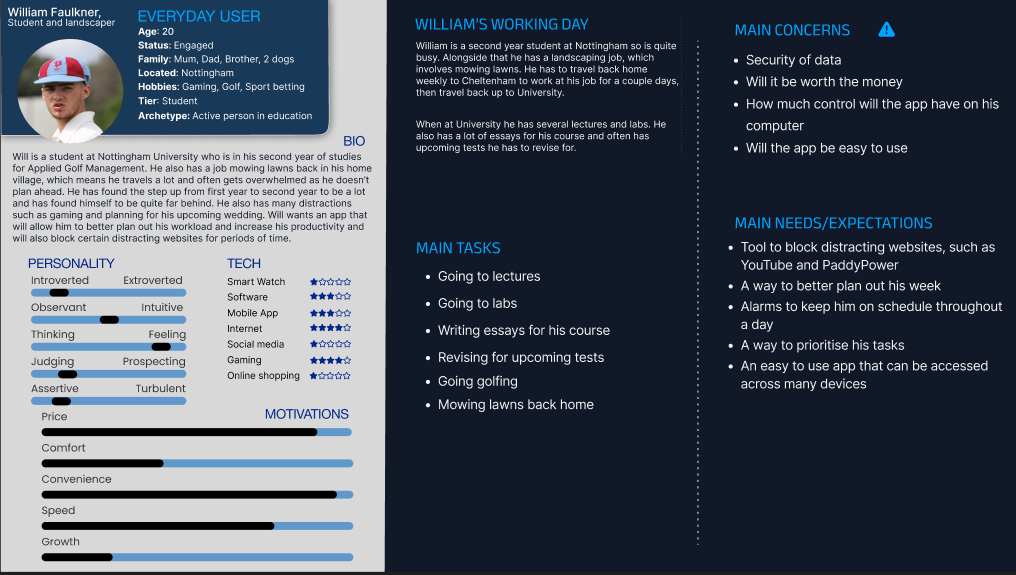
\includegraphics[width=0.92\textwidth]{./images/Persona_Matt.png}
	\caption*{} %最终文档中希望显示的图片标题
	\label{Fig.Persona3} %用于文内引用的标签
\end{figure}

\section{CI pipeline setup}

\begin{figure}[H] %H为当前位置,!htb为忽略美学标准,htbp为浮动图形
	\centering %图片居中
	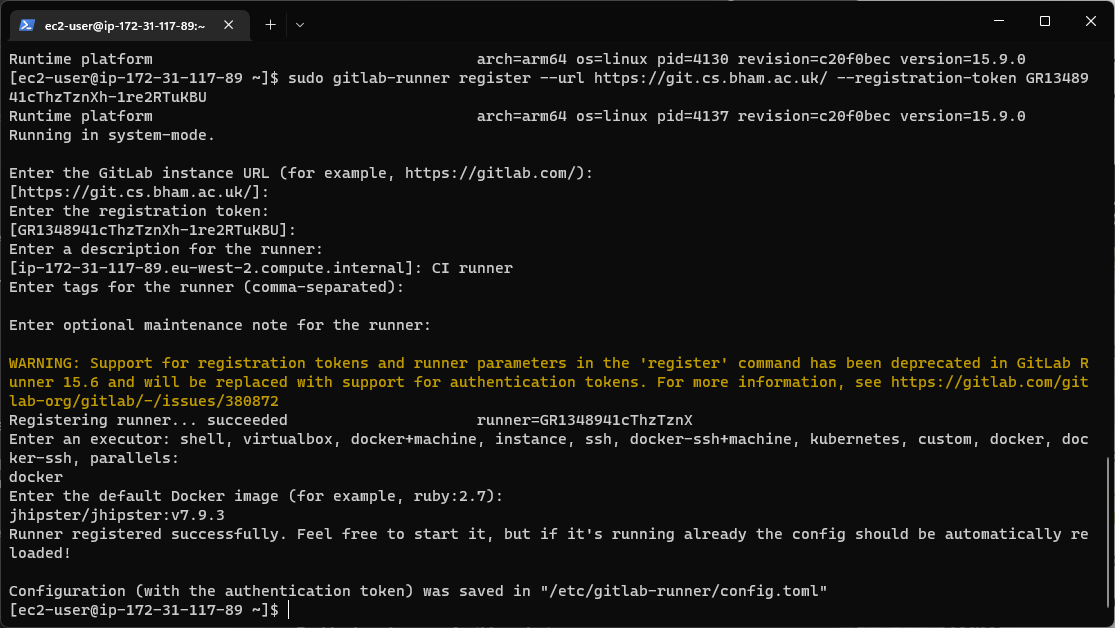
\includegraphics[width=0.84\textwidth]{./images/pipeline_install_gitlab_runner.png}
	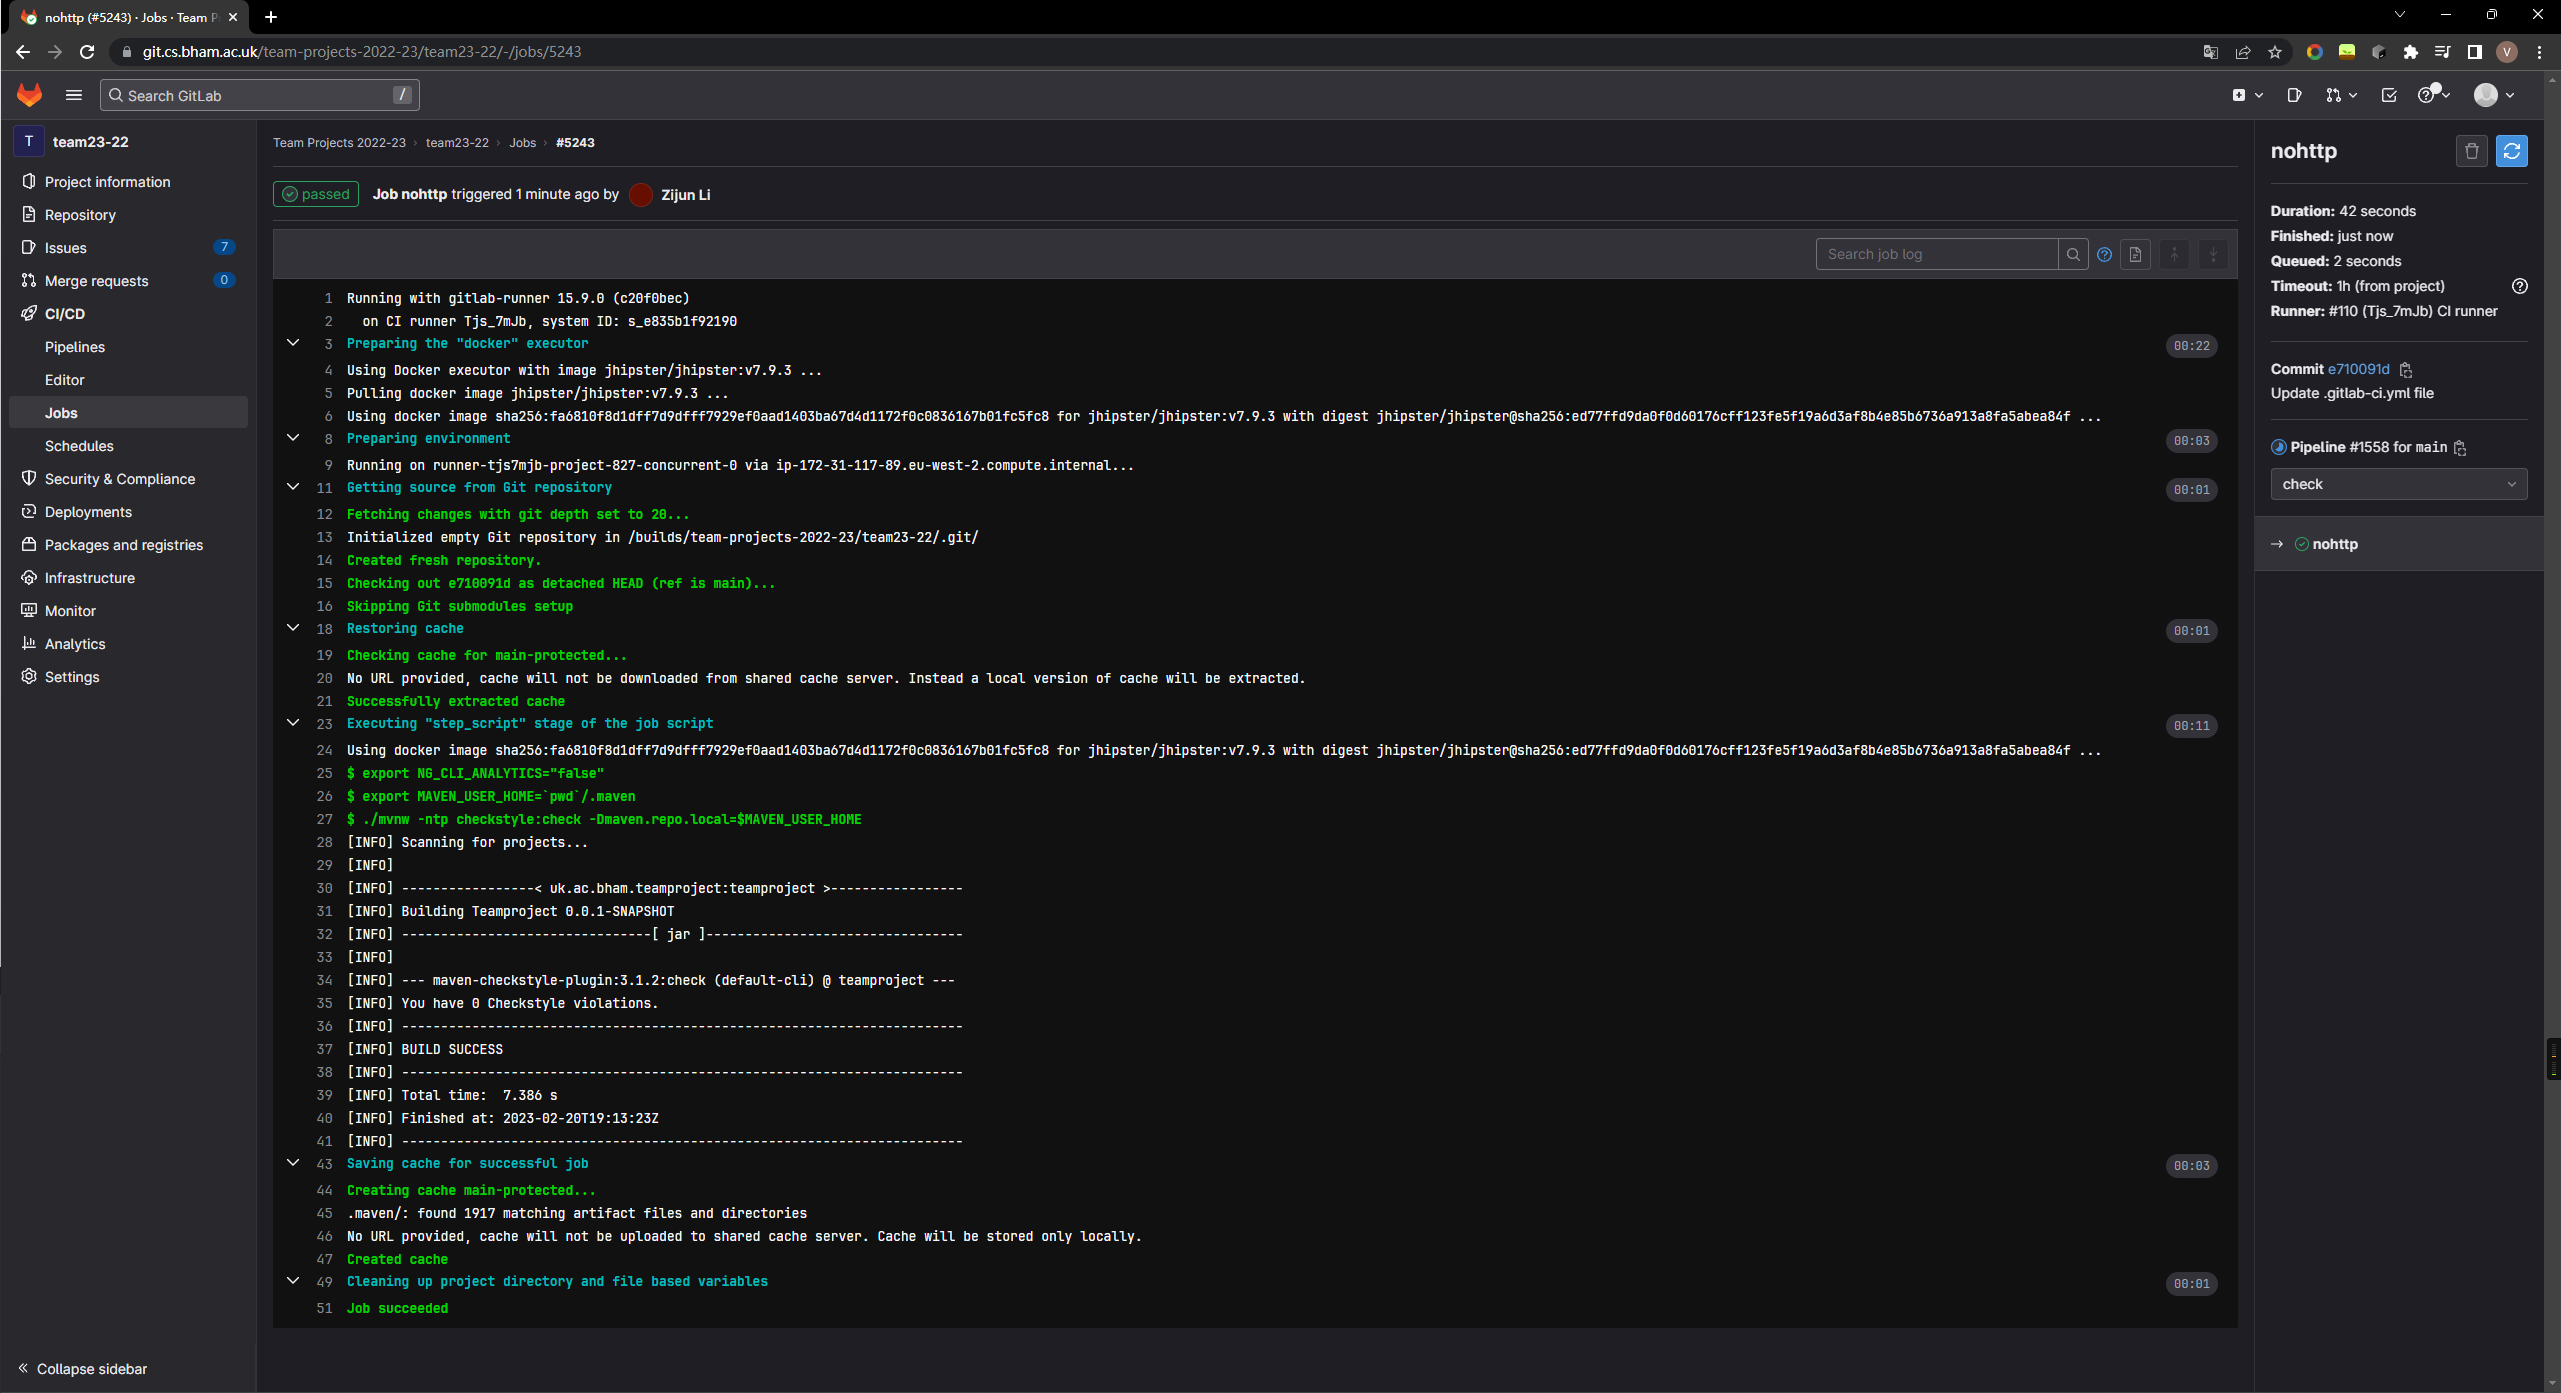
\includegraphics[width=0.84\textwidth]{./images/pipeline_work.png}
	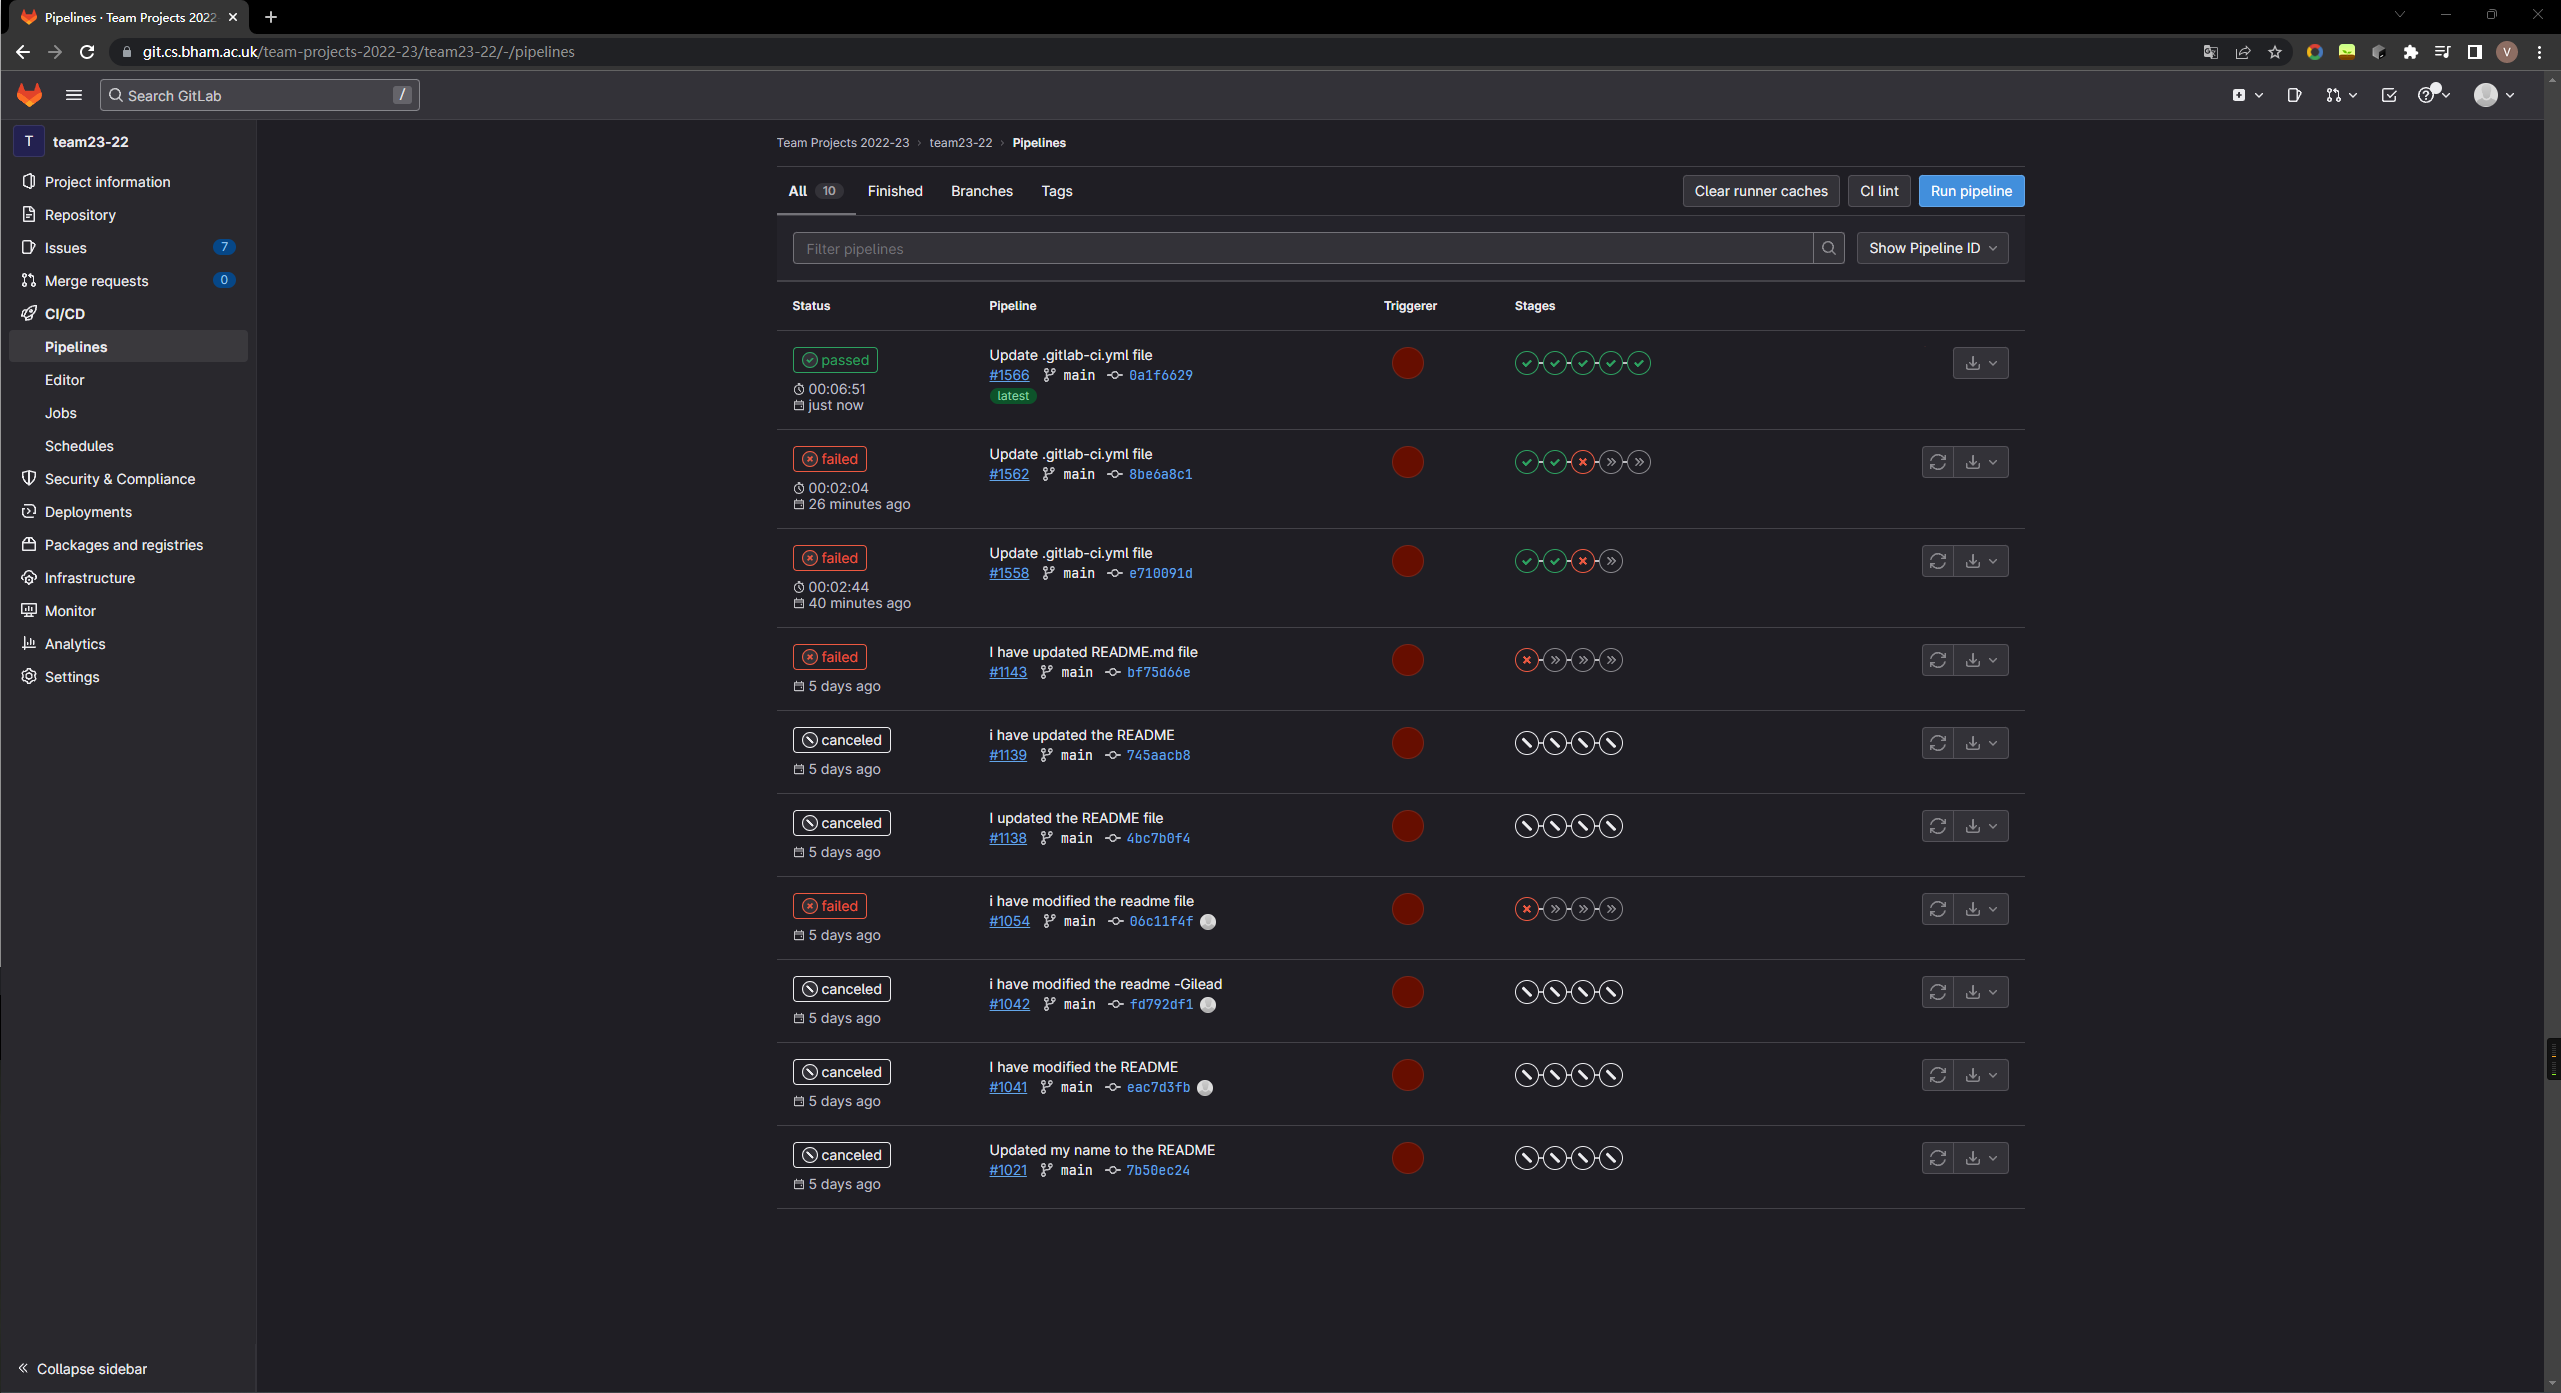
\includegraphics[width=0.84\textwidth]{./images/pipeline_success.png} %插入图片,[]中设置图片大小,{}中是图片文件名
	\caption*{CI pipeline} %最终文档中希望显示的图片标题
	\label{Fig.main2} %用于文内引用的标签
\end{figure}

\newpage

\section{Meeting diary}

{\noindent\begin{tabular}{|p{0.2\linewidth}|p{0.75\linewidth}|} 
	\hline
 \multicolumn{2}{|l|}{\textbf{Week 2: Meeting 1}}\\
 \hline
 \textbf{Date} & 10-2-2023\\
 \hline
 \textbf{Time} & 13:00-13:30(UK Time Zone)\\
 \hline
 \textbf{Venue} & Room 222\\
 \hline
 \multirow{2}*{\textbf{Attendees}} & Meeting Chair: Christian Vergara Marcillo\\
 ~ & Other Participants: Chance Egbon, Gilead Bempah, Matthew Goulding, Zijun Li, Bogdan-Marian Gheorghe\\
 \hline
 \multirow{3}*{\textbf{Discussions}} & - Only one team member was absent from our first meeting with the TA. We asked the TA for more details about the project, such as whether it should be a web application or a mobile application. We also discussed the application's viability, what we would be expected to do for it, and what each team member should submit for the S1. \\
 ~ & - The TA suggested that we combine the Time Management application and the Anti-Procrastination application because their goals were so similar. We also displayed our ideas for our team project application, which included applications for a care home, a murder mystery game, and an anti-procrastination tool. \\
 ~ & - The TA urged us to reduce the scope of the Anti-Procrastination programme to something that might block websites. Originally, we had suggested for the Anti-Procrastination application to be a piece of software that disabled applications on the user's PC until a timer expired. \\
 ~ & - The care home application caught the TA's attention because we suggested that it be both a phone app and a web application, with the website having the full experience and the phone app having less functionality. However, this would have required more work because we are creating both a phone app and a website. \\
 \hline
 \textbf{Decisions Made} & - We decided later in a call that we would put these ideas to a vote with a  form with the highest chosen being the one we would do, and the Anti-Procrastination/Time management application won, we also decided to host regular meetings with each other online using discord to stay up to date with each others progress.\\
 \hline
\end{tabular}}

\hspace*{\fill}\\

{\noindent\begin{tabular}{|p{0.2\linewidth}|p{0.75\linewidth}|} 
	\hline
 \multicolumn{2}{|l|}{\textbf{Week 3: Meeting 1}}\\
 \hline
 \textbf{Date} & 13-2-2023\\
 \hline
 \textbf{Time} & 16:00-16:30(UK Time Zone)\\
 \hline
 \textbf{Venue} & Discord Calls\\
 \hline
 \textbf{Attendees} & Participants: Chance Egbon, Samuel Okasia, Matthew Goulding, Zijun Li, Bogdan-Marian Gheorghe, Gilead Bempah, Smit Navinkumar\\
 \hline
 \multirow{2}*{\textbf{Discussions}} & - At this meeting, we spoke about the features that our application might offer. After coming up with about 7 or 8 features, we divided them up amongst ourselves according to who wanted to work on which feature. \\
 ~ & - We talked about the technology we would use to create our personas and mockups so that some degree of coherence would be achievable, and we then went on to work on our individual mockups for our submissions (Mockup, Persona, Kanban cards, etc...). \\
 \hline
 \textbf{Decisions Made} & - We chose to use the Figma tool for our mockups and Discord as our primary method of communication because it made it simpler for us to assist one another if any problems arose. If someone was having trouble with a particular aspect of S1, we could enter a video call and show our screens to help one another.\\
 \hline
\end{tabular}}

\hspace*{\fill}\\

{\noindent\begin{tabular}{|p{0.2\linewidth}|p{0.75\linewidth}|} 
	\hline
 \multicolumn{2}{|l|}{\textbf{Week 3: Meeting 2}}\\
 \hline
 \textbf{Date} & 14-2-2023\\
 \hline
 \textbf{Time} & 14:20-14:40(UK Time Zone)\\
 \hline
 \textbf{Venue} & Room 117\\
 \hline
 \multirow{2}*{\textbf{Attendees}} & Meeting Chair: Christian Vergara Marcillo \\
 ~ & Other Participants: Chance Egbon, Samuel Okasia, Matthew Goulding, Zijun Li, Bogdan-Marian Gheorghe \\
 \hline
 \textbf{Discussions} & - During the meeting, we asked TA for suggestions on the format of the mockups and personas.\\
 \hline
 \textbf{Decisions Made} & - TA provided some useful insights, including emphasizing the importance of including more detailed information in personas to make them more useful and realistic. The suggestion was also made to use standard templates for both mockups and personas to ensure consistency and clarity.\\
 \hline
\end{tabular}}

\hspace*{\fill}\\

{\noindent\begin{tabular}{|p{0.2\linewidth}|p{0.75\linewidth}|} 
	\hline
 \multicolumn{2}{|l|}{\textbf{Week 4: Meeting 1}}\\
 \hline
 \textbf{Date} & \makecell[l]{21-2-2023}\\
 \hline
 \textbf{Time} & \makecell[l]{14:20-14:40(UK Time Zone)}\\
 \hline
 \textbf{Venue} & \makecell[l]{Room 225}\\
 \hline
 \multirow{2}*{\textbf{Attendees}} & Meeting Chair: Christian Vergara Marcillo \\
 ~ & Other Participants: Matthew Goulding, Zijun Li, Smit Navinkumar, Gilead Bempah \\
 \hline
 \multirow{2}*{\textbf{Discussions}} & - We discussed the M1 team assessment during this meeting, and the TA provided more information about what we needed to complete before submitting. In particular, he spoke to us about our mockups and how we would need to remake them to be coherent with one another. He also advised us to start developing (coding) our application as soon as possible because it will give us more time to fix any errors we discover. He also suggested that we collaborate and determine among ourselves which database application we would utilise for our application. \\
 ~ & - We talked about how we would accomplish these goals after the meeting was over. \\
 \hline
 \textbf{Decisions Made} & - We changed the persona and mockup styles to the ones that received the greatest scores in the S1 ranking.\\
 \hline
\end{tabular}}

\section{S2 task allocation \& planning}

\subsection{Scheduler}

\begin{figure}[H] %H为当前位置,!htb为忽略美学标准,htbp为浮动图形
	\centering %图片居中
	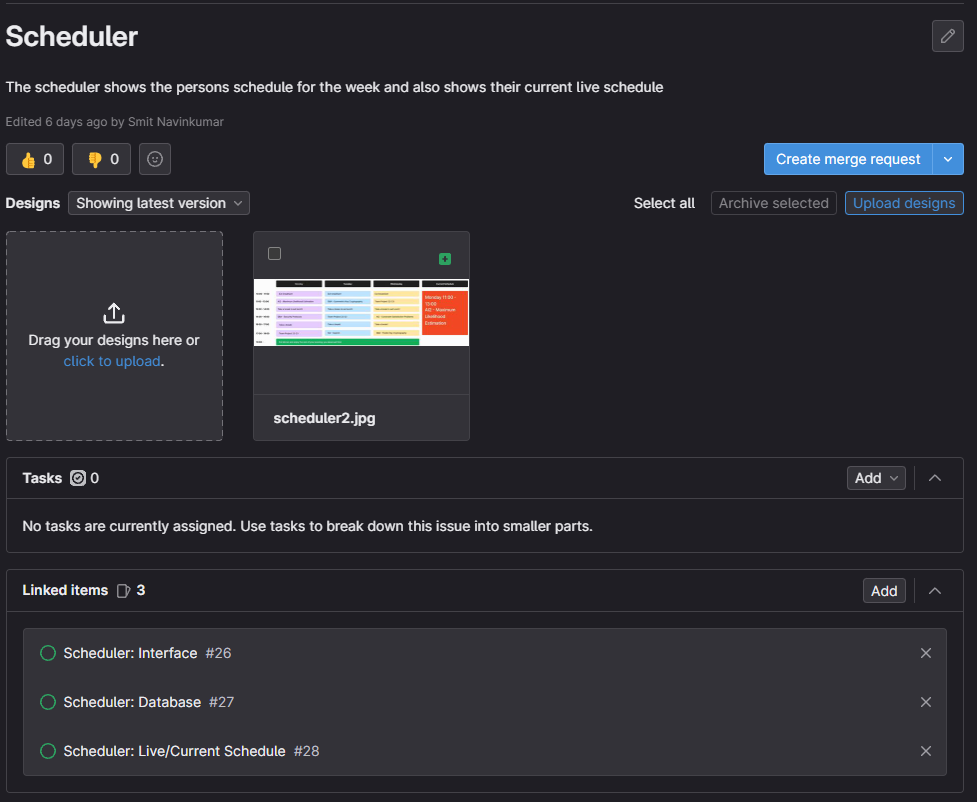
\includegraphics[width=0.85\textwidth]{./images/S2_Scheduler.png}
	\caption*{Smit} %最终文档中希望显示的图片标题
	\label{Fig.S2_Scheduler} %用于文内引用的标签
\end{figure}

\subsection{To-do List}

\begin{figure}[H] %H为当前位置,!htb为忽略美学标准,htbp为浮动图形
	\centering %图片居中
	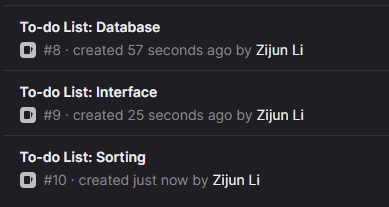
\includegraphics[width=0.85\textwidth]{./images/S2_To-do_List.png}
	\caption*{Zijun} %最终文档中希望显示的图片标题
	\label{Fig.S2_todo} %用于文内引用的标签
\end{figure}

\subsection{Anti-procrastination}

\begin{figure}[H] %H为当前位置,!htb为忽略美学标准,htbp为浮动图形
	\centering %图片居中
	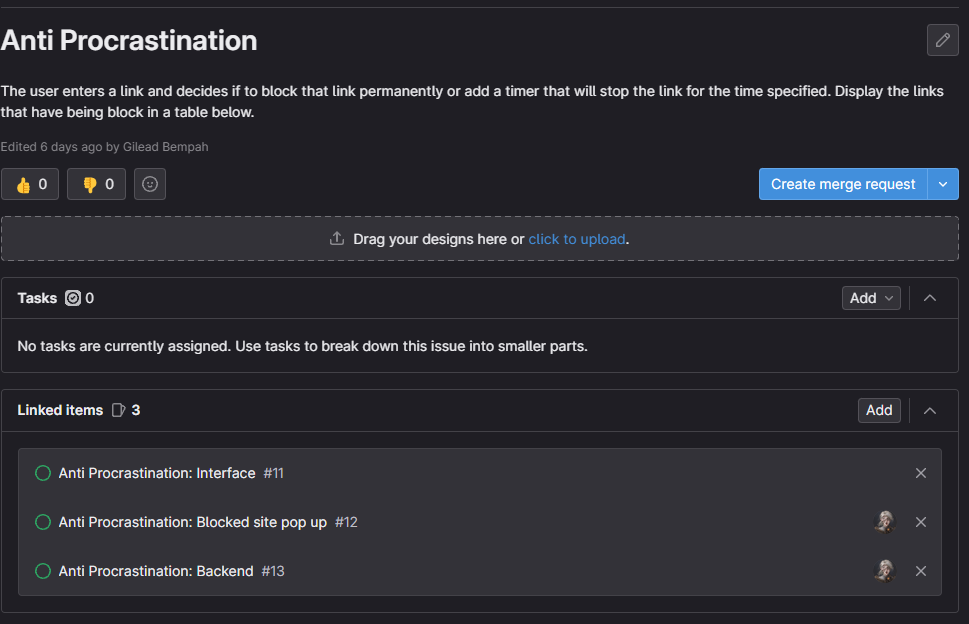
\includegraphics[width=0.85\textwidth]{./images/S2_Anti-Procrastination.png}
	\caption*{Gilead} %最终文档中希望显示的图片标题
	\label{Fig.S2_Anti-procrastination} %用于文内引用的标签
\end{figure}

\subsection{Diary}

\begin{figure}[H] %H为当前位置,!htb为忽略美学标准,htbp为浮动图形
	\centering %图片居中
	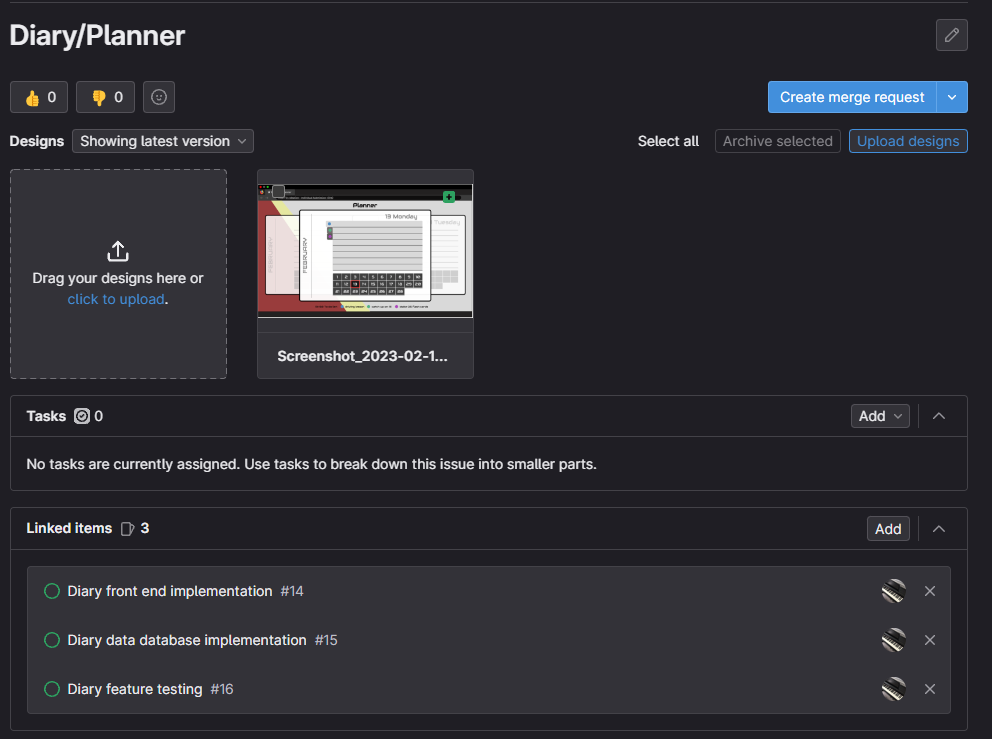
\includegraphics[width=0.85\textwidth]{./images/S2_Diary.png}
	\caption*{Chance} %最终文档中希望显示的图片标题
	\label{Fig.S2_Diary} %用于文内引用的标签
\end{figure}

\subsection{Alarm/Timer}

\begin{figure}[H] %H为当前位置,!htb为忽略美学标准,htbp为浮动图形
	\centering %图片居中
	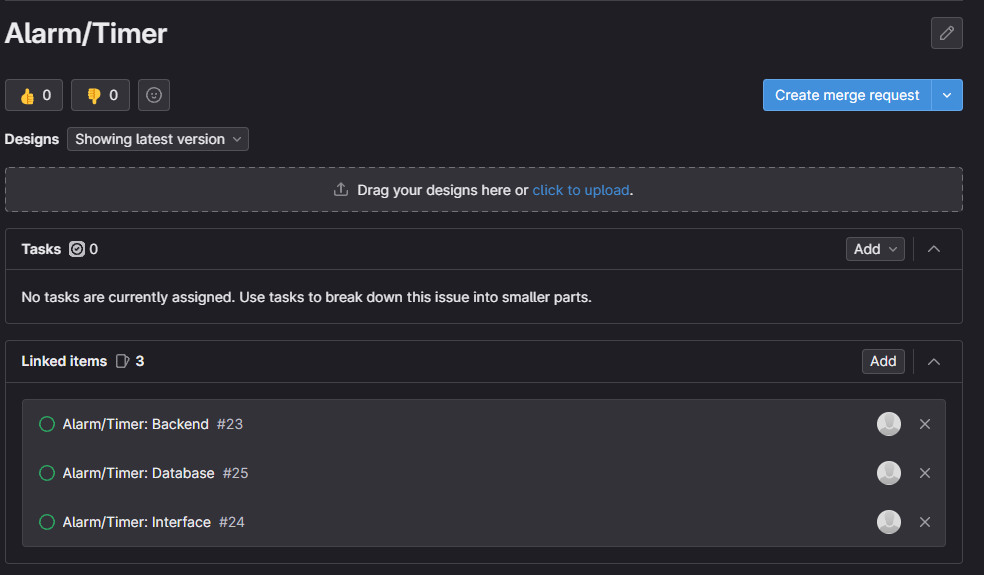
\includegraphics[width=0.76\textwidth]{./images/S2_Alarm.png}
	\caption*{Matthew} %最终文档中希望显示的图片标题
	\label{Fig.S2_Alarm} %用于文内引用的标签
\end{figure}

\subsection{Email notifications}

\begin{figure}[H] %H为当前位置,!htb为忽略美学标准,htbp为浮动图形
	\centering %图片居中
	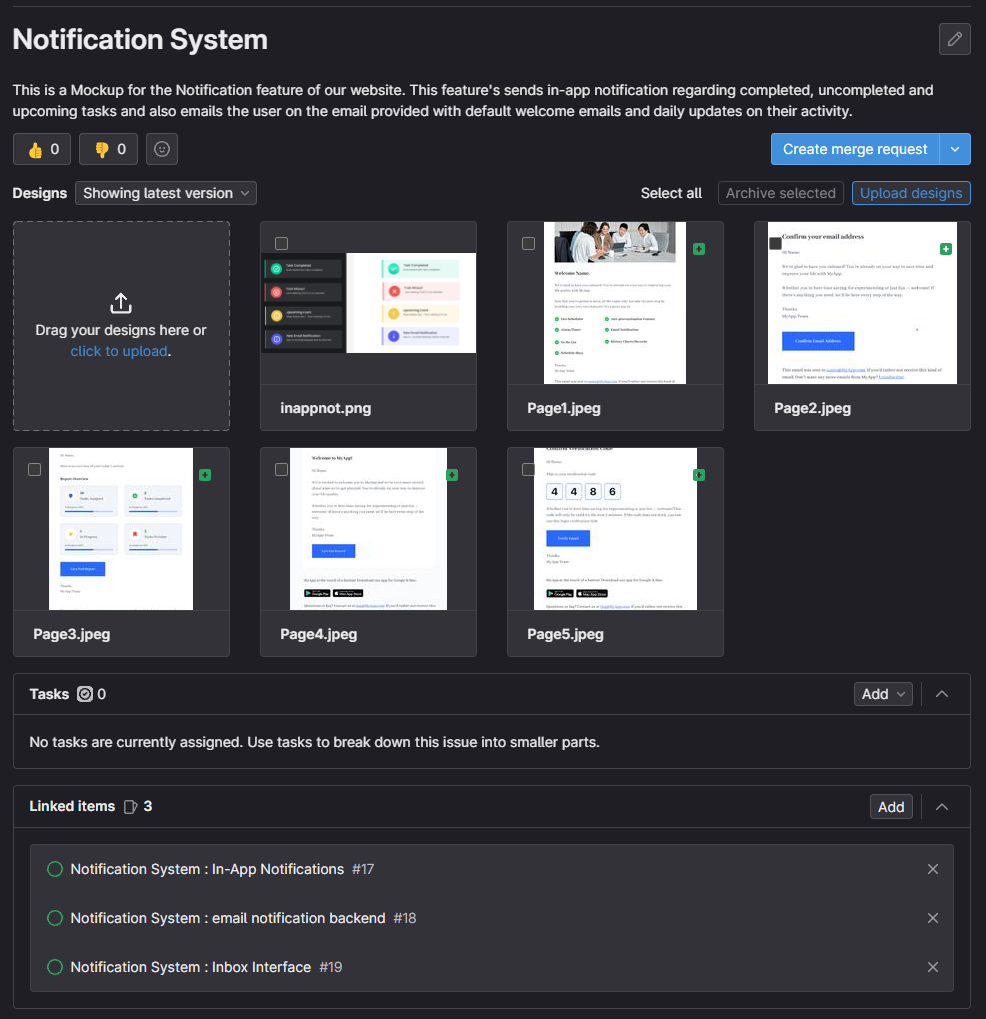
\includegraphics[width=0.76\textwidth]{./images/S2_Email.png}
	\caption*{Bogdan} %最终文档中希望显示的图片标题
	\label{Fig.S2_Email} %用于文内引用的标签
\end{figure}

\subsection{History}

\begin{figure}[H] %H为当前位置,!htb为忽略美学标准,htbp为浮动图形
	\centering %图片居中
	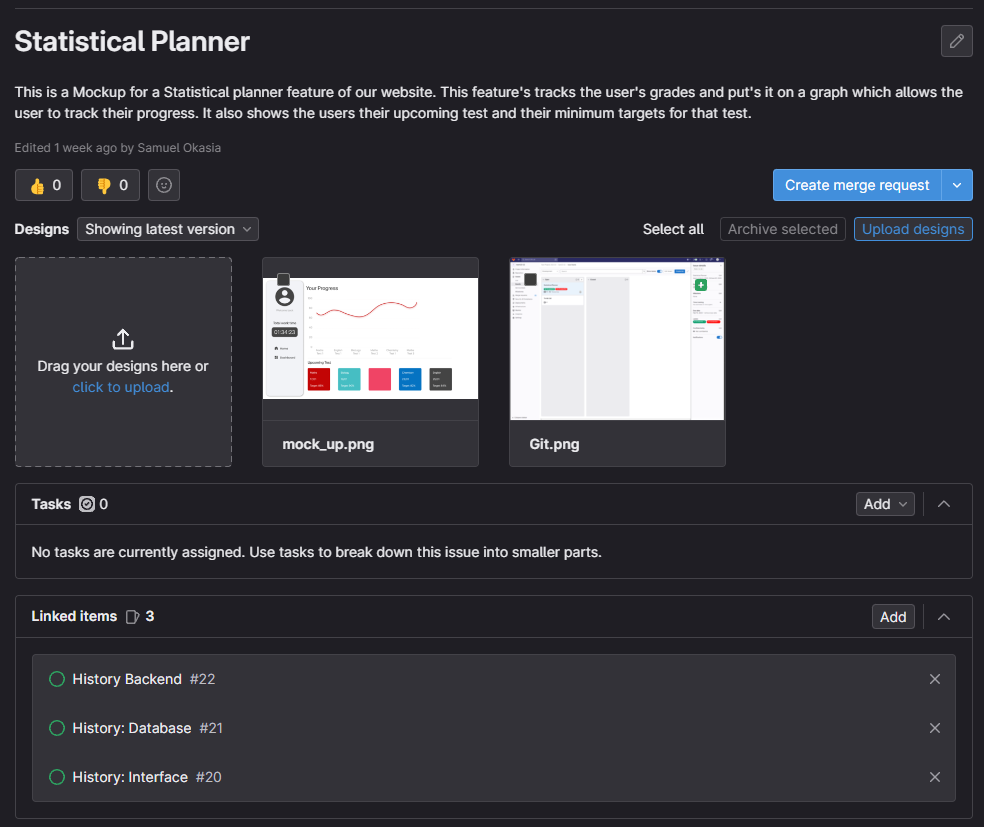
\includegraphics[width=0.85\textwidth]{./images/S2_History.png}
	\caption*{Samuel} %最终文档中希望显示的图片标题
	\label{Fig.S2_History} %用于文内引用的标签
\end{figure}

\end{document}